\documentclass[runningheads]{llncs}
\usepackage[T1]{fontenc}
\usepackage{graphicx}
\usepackage{booktabs}
\usepackage{longtable}
\usepackage{array}
\usepackage{amsmath}
\usepackage{amssymb}
\usepackage{xcolor}
\usepackage{hyperref}
\usepackage{calc}
% pandoc helpers
\providecommand{\tightlist}{\setlength{\itemsep}{0pt}\setlength{\parskip}{0pt}}
\providecommand{\pandocbounded}[1]{#1}
\usepackage{etoolbox}
% allow longtable inside LNCS
\begin{document}

\title{GPU-accelerated single-cell and spatial transcriptomics on NVIDIA DGX H100: a systematic benchmark of speed, scalability, and biological concordance}
\titlerunning{GPU-accelerated single-cell and spatial transcriptomics}

\author{Luca Vedovelli\inst{1,2} \and
Corrado Lanera\inst{1,2} \and
Daniele Sabbatini\inst{1,2,3} \and
Dario Gregori\inst{1,2}}

\authorrunning{L. Vedovelli et al.}

\institute{Unit of Biostatistics, Epidemiology and Public Health, Department of Cardiac, Thoracic, Vascular Sciences and Public Health, University of Padova, Padova, Italy \\
\email{\{luca.vedovelli,corrado.lanera,daniele.sabbatini,dario.gregori\}@ubep.unipd.it} \and
BIOSTAT-X, Biostatistics \& AI for Biomedical Discovery, Pediatric Research Institute ``Citt\`a della Speranza'', Padova, Italy \and
Neuromuscular Unit, Department of Neuroscience, University of Padua, Padua, Italy}

\maketitle

\begin{abstract}
Single-cell RNA sequencing (scRNA-seq) datasets now routinely exceed one million cells, and spatial transcriptomics platforms such as Visium HD generate hundreds of thousands of measurement bins per tissue section, placing severe computational demands on analysis frameworks that remain predominantly CPU-bound. We present a systematic benchmark comparing Scanpy (CPU, 100 cores) against rapids-singlecell (GPU, 1--8 NVIDIA H100 80~GB) on the 1.3-million mouse brain cell dataset, evaluating speed, multi-GPU scalability, memory efficiency, and biological concordance across five dataset sizes (10k--1.3M cells) with five independent repeats. The GPU pipeline achieved up to 120-fold end-to-end speedup at 1.3M cells (435~s vs 52,056~s on CPU), reducing a 14.5-hour analysis to 7.3~minutes. Biological concordance was high: HVG selection was identical (Jaccard~=~1.0), PCA loadings perfectly correlated (Spearman~$|\rho|$~=~1.0), and Leiden clustering concordance ranged from ARI~=~0.908 to 0.963. Multi-GPU scaling was sublinear due to CPU preprocessing dominance. A memory-optimised pipeline processed 11.9 million cells on a single DGX H100 node, with CPU RAM as the binding constraint (GPU VRAM at 7.6\% of capacity). A differential expression benchmark at 3.4M cells showed pseudo-bulk aggregation 44$\times$ faster than cell-level t-test. We extended the benchmark to spatial transcriptomics on three 10x Visium platforms, achieving up to 51.6$\times$ end-to-end speedup (Visium HD 8~$\mu$m) and 3,272$\times$ for co-occurrence analysis, with near-perfect spatial autocorrelation concordance (Spearman~$\rho \geq 0.9995$). These results identify CPU-side preprocessing as the primary bottleneck and provide practical guidance for deploying GPU-accelerated workflows at atlas scale.

\keywords{GPU computing \and single-cell RNA-seq \and spatial transcriptomics \and benchmarking \and rapids-singlecell}
\end{abstract}

\section{Introduction}\label{introduction}

Single-cell RNA sequencing has become the standard technology for
dissecting cellular heterogeneity in complex tissues \citep{Regev2017}.
Recent atlas-scale projects such as the Human Cell Atlas
\citep{Regev2017}, Tabula Sapiens \citep{TabulaSapiens2022}, and the
Allen Brain Atlas \citep{Yao2023} routinely generate datasets ranging
from hundreds of thousands to millions of cells, placing severe
computational demands on analysis pipelines. The dominant analysis
framework, Scanpy \citep{Wolf2018}, executes on CPU and relies on NumPy,
SciPy, and scikit-learn for linear algebra and graph operations. While
multi-threaded CPU implementations scale modestly with core count, a
standard analysis of one million cells, encompassing quality control,
normalisation, principal component analysis (PCA), neighbourhood graph
construction, Leiden clustering \citep{Traag2019}, uniform manifold
approximation and projection (UMAP) \citep{McInnes2018}, and
differential expression (DE) testing, can require hours to days on a
multi-core workstation.

In parallel, spatial transcriptomics has matured from low-throughput
technologies to platforms that tile entire tissue sections with hundreds
of thousands of measurement points. The 10x Genomics Visium HD platform
generates up to 6.3 million 2 um bins per tissue section, and spatial
analysis pipelines built on Squidpy \citep{Palla2022} add
computationally intensive operations such as spatial autocorrelation
(Moran's I, Geary's C), co-occurrence analysis, and neighbourhood
enrichment on top of the standard expression analysis workflow. As both
single-cell and spatial datasets grow, the need for GPU-accelerated
analysis becomes increasingly pressing.

GPU-accelerated alternatives have emerged to address this scalability
challenge. The RAPIDS ecosystem \citep{RAPIDS2024} provides GPU-native
implementations of common data science primitives, and rapids-singlecell
\citep{Dicks2026} offers a near-drop-in replacement for Scanpy that
executes the same analytical pipeline on NVIDIA GPUs via cuML, cuGraph,
and CuPy. Prior work has demonstrated substantial GPU speedups for
genomic analyses \citep{TaylorWeiner2019}, including single-cell
pipelines \citep{Nolet2022}, and proposed GPU frameworks for datasets
exceeding ten million cells \citep{Hu2025}. However, most benchmarks
report headline speedups without systematically examining (i) per-step
performance variation, (ii) multi-GPU scaling behaviour and its
bottlenecks, (iii) numerical concordance of GPU floating-point results
with CPU baselines, and (iv) practical memory limits at extreme scale.
Gardner et al. \citeyearpar{Gardner2025} recently evaluated
accuracy-performance trade-offs for GPU single-cell analysis, but their
study was limited to a single GPU and did not explore multi-GPU
configurations or stress-test hardware limits.

Here we present a comprehensive benchmark addressing five questions
simultaneously. First, speed: what is the per-step and end-to-end
speedup of rapids-singlecell relative to Scanpy on identical hardware?
Second, scalability: how does the pipeline scale from 1 to 8 GPUs (the
full GPU complement of a single NVIDIA DGX H100 node), and where are the
bottlenecks? Third, concordance: do CPU and GPU pipelines yield
biologically equivalent results in terms of HVG selection, PCA
embeddings, clustering, and DE gene rankings? Fourth, capacity: what is
the maximum dataset size a single DGX H100 node can process, and what
limits it? Fifth, spatial generalisability: do the GPU speedup and
concordance patterns extend from single-cell to spatial transcriptomics?

We benchmark both modalities on NVIDIA DGX H100 and RTX 4090 hardware,
provide all code and containers for full reproducibility, and identify
CPU-side preprocessing as the primary bottleneck limiting further
scaling.

\section{Data and Methods}\label{data-and-methods}

\subsection{Single-cell RNA-seq}\label{single-cell-rna-seq}

\subsubsection{Dataset and subsampling}\label{dataset-and-subsampling}

All single-cell experiments used the 10x Genomics 1.3-million mouse
brain cell dataset (E18) \citep{Zheng2017}, obtained as a pre-processed
AnnData h5ad file from the RAPIDS single-cell examples repository. This
dataset is the canonical large-scale single-cell benchmark and contains
approximately 1.3 million cells with gene expression measured by the 10x
Chromium platform.

To evaluate performance across scales, we created reproducible
subsamples of 10,000, 50,000, 100,000, and 500,000 cells by uniform
random sampling without replacement (\texttt{numpy.random.choice}, NumPy
2.2.6, seed = 42), in addition to the full 1.3M cell dataset. All
subsamples were derived from the same parent dataset to ensure
consistent biological composition across benchmarking tiers.

\subsubsection{Analysis pipeline}\label{analysis-pipeline}

Both the CPU and GPU pipelines implemented the standard Scanpy
best-practices workflow \citep{Luecken2019, Heumos2023} with identical
parameters. The CPU pipeline used Scanpy 1.12 \citep{Wolf2018} with
NumPy 2.2.6 and the igraph Leiden backend (igraph 1.0.0); the GPU
pipeline used rapids-singlecell 0.14.1 \citep{Dicks2026} with CuPy
13.6.0, the RAPIDS Memory Manager (RMM) 26.2.0, and the cuGraph Leiden
backend. Both pipelines shared the AnnData format \citep{Virshup2024}
for data interchange.

The pipeline comprised ten steps, each timed independently using
\texttt{time.perf\_counter()} (Table 1).

\begin{longtable}[]{@{}
  >{\raggedleft\arraybackslash}p{(\linewidth - 6\tabcolsep) * \real{0.1111}}
  >{\raggedright\arraybackslash}p{(\linewidth - 6\tabcolsep) * \real{0.2037}}
  >{\raggedright\arraybackslash}p{(\linewidth - 6\tabcolsep) * \real{0.2963}}
  >{\raggedright\arraybackslash}p{(\linewidth - 6\tabcolsep) * \real{0.3889}}@{}}
\caption{\textbf{Table 1.} Pipeline steps, parameters, and
implementations for the scRNA-seq benchmark. All steps used identical
parameters for the CPU and GPU pipelines except where
noted.}\label{tbl:pipeline}\tabularnewline
\toprule\noalign{}
\begin{minipage}[b]{\linewidth}\raggedleft
Step
\end{minipage} & \begin{minipage}[b]{\linewidth}\raggedright
Operation
\end{minipage} & \begin{minipage}[b]{\linewidth}\raggedright
Key parameters
\end{minipage} & \begin{minipage}[b]{\linewidth}\raggedright
Implementation note
\end{minipage} \\
\midrule\noalign{}
\endfirsthead
\toprule\noalign{}
\begin{minipage}[b]{\linewidth}\raggedleft
Step
\end{minipage} & \begin{minipage}[b]{\linewidth}\raggedright
Operation
\end{minipage} & \begin{minipage}[b]{\linewidth}\raggedright
Key parameters
\end{minipage} & \begin{minipage}[b]{\linewidth}\raggedright
Implementation note
\end{minipage} \\
\midrule\noalign{}
\endhead
\bottomrule\noalign{}
\endlastfoot
1 & Data loading & --- & \texttt{read\_h5ad()} from disk \\
2 & QC and filtering & \texttt{min\_genes} = 200, \texttt{min\_cells} =
3, mt prefix = \texttt{mt-} & Mitochondrial percentage calculated,
cells/genes filtered \\
3 & Normalisation & \texttt{target\_sum} = 10,000 & Library-size scaling
+ \texttt{log1p} \\
4 & HVG selection & \texttt{n\_top\_genes} = 2,000, Seurat v1 method &
On log-normalised data \citep{Satija2015, Yip2019} \\
5 & Scaling & \texttt{max\_value} = 10 & Sparse to dense float32,
mean-centre, unit-variance \\
6 & PCA & 50 components, seed = 42 & Truncated SVD \\
7 & Neighbour graph & k = 15, 50 PCs, seed = 42 & k-NN in PCA space \\
8 & Leiden clustering & r in \{0.5, 1.0, 1.5\}, seed = 42 & igraph (CPU)
/ cuGraph (GPU) \citep{Traag2019} \\
9 & UMAP & 2 components, seed = 42 & 2D embedding \citep{McInnes2018} \\
10 & DE testing & Wilcoxon, one-vs-rest, \texttt{use\_raw} = True & On
Leiden r = 1.0 clusters \citep{Soneson2018} \\
\end{longtable}

For the CPU pipeline, threading was maximised by setting
\texttt{OMP\_NUM\_THREADS}, \texttt{MKL\_NUM\_THREADS},
\texttt{OPENBLAS\_NUM\_THREADS}, and \texttt{NUMBA\_NUM\_THREADS} to 100
(the usable core count) before importing any numerical library. These
variables target the thread pools of four distinct parallel backends
that NumPy, SciPy, scikit-learn, and UMAP may dispatch to: OpenMP (used
by OpenBLAS and several \texttt{sklearn} inner loops), Intel MKL,
OpenBLAS, and Numba (the JIT backend of \texttt{umap-learn}). Only the
pool corresponding to the BLAS library that NumPy was linked against at
build time is actually active at runtime; the other variables are
harmlessly ignored. We set all four to remain portable across container
variants where the BLAS choice may differ; in our RAPIDS base image,
NumPy is linked against OpenBLAS. For single-GPU runs, the RMM pool
allocator was initialised to pre-reserve GPU VRAM and amortise
allocation cost across many small operations; a GPU warmup step was then
executed to absorb CUDA context initialisation overhead before timing.

\subsubsection{Multi-GPU pipeline}\label{multi-gpu-pipeline}

For datasets exceeding single-GPU VRAM capacity (500k and 1.3M cells),
we employed a hybrid multi-GPU pipeline using Dask-CUDA
\citep{Rocklin2015}. Preprocessing steps (data loading, QC,
normalisation, HVG selection) executed on CPU, as they are I/O- or
memory-bound and do not benefit from GPU parallelism. PCA and neighbour
graph construction were distributed across N GPUs (N in \{2, 4, 8\}) via
Dask workers, each with a 10 GB initial / 70 GB maximum RMM pool.
Scaling, Leiden clustering, UMAP, and DE testing executed on a single
GPU (device 0), as they operate on the reduced PCA embedding or require
global graph access.

\subsubsection{Concordance metrics}\label{concordance-metrics}

To assess whether the GPU pipeline produces biologically equivalent
results, we selected six concordance metrics, one for each major stage
of the analysis pipeline, such that a divergence at any stage would be
detected independently of the others (Table 2). The panel follows the
metric families adopted in published scRNA-seq method benchmarks
\citep{Tian2019, Duo2020, Luecken2022}, progressing from deterministic
upstream operations (feature selection, dimensionality reduction)
through graph and clustering steps to downstream differential
expression.

\begin{longtable}[]{@{}
  >{\raggedright\arraybackslash}p{(\linewidth - 4\tabcolsep) * \real{0.2963}}
  >{\raggedright\arraybackslash}p{(\linewidth - 4\tabcolsep) * \real{0.4444}}
  >{\raggedright\arraybackslash}p{(\linewidth - 4\tabcolsep) * \real{0.2593}}@{}}
\caption{\textbf{Table 2.} Concordance metrics used to compare CPU and
GPU pipeline outputs.}\label{tbl:concordance}\tabularnewline
\toprule\noalign{}
\begin{minipage}[b]{\linewidth}\raggedright
Metric
\end{minipage} & \begin{minipage}[b]{\linewidth}\raggedright
Definition
\end{minipage} & \begin{minipage}[b]{\linewidth}\raggedright
Scope
\end{minipage} \\
\midrule\noalign{}
\endfirsthead
\toprule\noalign{}
\begin{minipage}[b]{\linewidth}\raggedright
Metric
\end{minipage} & \begin{minipage}[b]{\linewidth}\raggedright
Definition
\end{minipage} & \begin{minipage}[b]{\linewidth}\raggedright
Scope
\end{minipage} \\
\midrule\noalign{}
\endhead
\bottomrule\noalign{}
\endlastfoot
HVG Jaccard & size of intersection divided by size of union of the CPU
and GPU gene sets for 2,000 HVGs & Feature selection \\
PCA loading & rho & \\
kNN Jaccard & Mean per-cell Jaccard overlap of k-nearest-neighbour sets
(k = 15) \citep{Luecken2022} & Graph structure \\
ARI & Adjusted Rand Index of Leiden cluster assignments, adjusted for
chance \citep{Hubert1985} & Clustering \\
NMI & Normalised Mutual Information of cluster assignments
\citep{Vinh2010} & Clustering \\
DE logFC rho & Spearman rho of log-fold-changes for top 100 DE genes per
cluster, after Hungarian matching \citep{Soneson2018} & Differential
expression \\
\end{longtable}

\subsubsection{Stress test: maximum
capacity}\label{stress-test-maximum-capacity}

To determine the maximum dataset size processable on a single DGX H100
node, we implemented a memory-optimised pipeline variant. The key
optimisations were: (i) scaling on CPU rather than GPU (leveraging 2 TB
system RAM); (ii) a distributed covariance PCA that scatters the scaled
matrix across all 8 GPUs, computes per-GPU partial covariance matrices
(each 2,000 x 2,000), sums and eigendecomposes on GPU 0, then projects
locally, which is mathematically equivalent to standard PCA via the
covariance method; (iii) lean GPU transfer that replaces the dense
matrix with an empty sparse placeholder after PCA, since downstream
steps (neighbours, clustering, UMAP) only require the PCA embedding; and
(iv) a reduced RMM pool (2 GB per worker). We conducted a binary search
from 3.4M to 13.7M cells to identify the failure point.

\subsubsection{Differential expression at
scale}\label{differential-expression-at-scale}

Differential expression testing at atlas scale is constrained by
hardware, which shaped the factorial design of this benchmark. At 3.4
million cells and 41,000 genes the raw count matrix
(\texttt{adata.raw.X}) occupies approximately 121 GB in sparse CSR
format, exceeding the 80 GB VRAM of any single H100 device; running GPU
DE naively is therefore impossible, and the tests we benchmark either
scatter genes across multiple GPUs or stream gene chunks through a
single GPU. We evaluated seven DE strategies in a factorial design
crossing test type (Wilcoxon, t-test, pseudo-bulk) with GPU strategy
(none, scatter-by-genes across 8 GPUs, chunk-and-stream on 1 GPU). Gene
chunks of 500 were used for GPU strategies, giving 500 x 3.4M x 4 bytes
approximately 6.8 GB per chunk, well within the 80 GB per-device limit.
Pseudo-bulk aggregation summed raw counts by donor x cluster, normalised
to counts per million, log-transformed, and applied the Wilcoxon test on
the aggregated matrix \citep{Squair2021}.

\subsection{Spatial transcriptomics}\label{spatial-transcriptomics}

\subsubsection{Datasets}\label{datasets}

Spatial benchmarks used two 10x Genomics public datasets, both
downloaded programmatically from the 10x Genomics public data portal.
The first is Visium v1 Mouse Brain Sagittal Anterior, the standard
spot-based spatial transcriptomics platform, consisting of 2,695 spots
at 55 um resolution and approximately 32,285 genes. The second is Visium
HD Mouse Brain (CytAssist, FFPE), benchmarked at two bin sizes: 8 um
(393,543 bins) and 2 um (subsampled from the native 6.3 million down to
389,492 bins), each quantifying 19,059 genes. The Visium HD 2 um dataset
was subsampled to approximately 400,000 bins using the
\texttt{-\/-max-spots} flag so that the benchmark would fit within the
RTX 4090's 24 GB VRAM; full-scale analysis of the complete 6.3 million
bins requires DGX-class resources.

\subsubsection{Spatial analysis
pipeline}\label{spatial-analysis-pipeline}

The spatial pipeline comprised two phases: an expression analysis phase
(shared with the scRNA-seq pipeline) and a spatial statistics phase
(Table 3).

\begin{longtable}[]{@{}
  >{\raggedleft\arraybackslash}p{(\linewidth - 6\tabcolsep) * \real{0.1622}}
  >{\raggedright\arraybackslash}p{(\linewidth - 6\tabcolsep) * \real{0.2973}}
  >{\centering\arraybackslash}p{(\linewidth - 6\tabcolsep) * \real{0.3514}}
  >{\raggedright\arraybackslash}p{(\linewidth - 6\tabcolsep) * \real{0.1892}}@{}}
\caption{\textbf{Table 3.} Spatial analysis pipeline steps. Steps 1-8
share parameters with the scRNA-seq pipeline (Table 1) except for QC
filtering, which used \protect\texttt{min\_genes} = 1 for Visium HD
(Space Ranger pre-filters on-tissue barcodes). Steps 9-14 are
spatial-specific.}\label{tbl:spatial_pipeline}\tabularnewline
\toprule\noalign{}
\begin{minipage}[b]{\linewidth}\raggedleft
Step
\end{minipage} & \begin{minipage}[b]{\linewidth}\raggedright
Operation
\end{minipage} & \begin{minipage}[b]{\linewidth}\centering
GPU support
\end{minipage} & \begin{minipage}[b]{\linewidth}\raggedright
Notes
\end{minipage} \\
\midrule\noalign{}
\endfirsthead
\toprule\noalign{}
\begin{minipage}[b]{\linewidth}\raggedleft
Step
\end{minipage} & \begin{minipage}[b]{\linewidth}\raggedright
Operation
\end{minipage} & \begin{minipage}[b]{\linewidth}\centering
GPU support
\end{minipage} & \begin{minipage}[b]{\linewidth}\raggedright
Notes
\end{minipage} \\
\midrule\noalign{}
\endhead
\bottomrule\noalign{}
\endlastfoot
1-8 & Expression analysis (QC through UMAP) & Yes & As in Table 1;
Leiden r = 1.0 for Visium, r = 0.1 for HD \\
9 & Spatial neighbours & No & Delaunay triangulation (scipy.spatial) \\
10 & Moran's I & Yes & Spatial autocorrelation per gene \\
11 & Geary's C & Yes & Spatial autocorrelation per gene \\
12 & Co-occurrence & Yes & Cluster co-occurrence across distance
intervals \\
13 & Neighbourhood enrichment & No & Cluster-cluster proximity
enrichment \\
14 & Ligand-receptor interaction & No & Cell communication inference \\
\end{longtable}

The CPU baseline used Scanpy 1.12 for expression steps and Squidpy 1.8.1
\citep{Palla2022} for spatial steps. The GPU pipeline used
rapids-singlecell 0.14.1 for both expression and GPU-accelerated spatial
steps (Moran's I, Geary's C, co-occurrence). Steps without GPU
implementations (spatial neighbours, neighbourhood enrichment,
ligand-receptor) were executed identically on CPU in both pipelines.

Co-occurrence and neighbourhood enrichment were skipped when cluster
counts exceeded 500, as their O(k\^{}2) memory complexity becomes
prohibitive. Ligand-receptor interaction analysis was skipped for
datasets exceeding 100,000 spots.

\subsubsection{Spatial concordance
metrics}\label{spatial-concordance-metrics}

We compared CPU and GPU spatial outputs along four complementary axes.
Spatial autocorrelation concordance was measured as the Spearman rho
between CPU and GPU per-gene Moran's I (and separately Geary's C)
statistics across all genes. Spatially variable gene (SVG) Jaccard
overlap was computed for the top-N SVGs ranked by Moran's I (with N
taking the values 50, 100, and 200) and for the complete set of genes
passing FDR \textless{} 0.05. Clustering agreement was assessed by the
adjusted Rand index and normalised mutual information of Leiden cluster
assignments from the expression-based pipeline. Finally, co-occurrence
concordance was the Spearman rho between the full CPU and GPU
co-occurrence matrices.

\subsection{Hardware and software
environment}\label{hardware-and-software-environment}

Single-cell benchmarks ran on a single node of the UPSCALE/CONVECS DGX
H100 cluster at the University of Padova, comprising 8 x NVIDIA H100 80
GB SXM GPUs connected via NVLink 4.0, dual Intel Xeon Platinum 8480C
CPUs (112 cores total), and 2 TB DDR5 RAM. The software environment was
encapsulated in a Singularity container built from the NVIDIA RAPIDS
base image (\texttt{nvcr.io/nvidia/rapidsai/base:26.02-cuda12-py3.12}).
Key software versions: Scanpy 1.12, rapids-singlecell 0.14.1, CuPy
13.6.0, Dask 2026.1.1, Dask-CUDA 26.2.0, Python 3.12.12. Jobs were
submitted via SLURM on a dedicated DGX H100 node (\texttt{poddgx02}).

Spatial benchmarks ran on a local workstation equipped with an NVIDIA
RTX 4090 (24 GB GDDR6X), 100 CPU cores, and 256 GB DDR5 RAM, driven by a
more recent NVIDIA driver (550.x). The spatial container was built on
the same \texttt{nvcr.io/nvidia/rapidsai/base:26.02-cuda12-py3.12} image
as the scRNA-seq container, with Squidpy 1.8.1 \citep{Palla2022} and
spatialdata \citep{Marconato2024} added on top for the spatial pipeline.
DGX-scale spatial benchmarks were not feasible within the study
timeline: although the scRNA pipeline executed successfully on the DGX
node via CUDA forward-compatibility, the GPU components of the spatial
pipeline failed on the cluster's driver (535.183.01), which caps CUDA
runtime at 12.2. We attempted to downgrade the spatial container to an
earlier RAPIDS release known to be driver-compatible (RAPIDS 25.02), but
the spatial dependency stack (rapids-singlecell 0.14, Squidpy
GPU-backend, spatialdata) could not be resolved against the older RAPIDS
wheels. Porting the full spatial pipeline to a driver-compatible RAPIDS
release therefore remains future work.

Each benchmark configuration was repeated five times; we report mean +/-
standard deviation. For spatial benchmarks, the first repeat served as a
JIT/warmup run and was excluded; we report the mean of repeats 2-5.

\subsection{Reproducibility}\label{reproducibility}

All code, Dockerfiles, SLURM submission scripts, and result JSON files
are available at \url{https://github.com/lucavd/2026.scRNA_DGX}. All
benchmarks ran in Python 3.12 inside a Singularity container built from
the Docker image \texttt{lucavd/sc-benchmark:latest} (base image
\texttt{nvcr.io/nvidia/rapidsai/base:26.02-cuda12-py3.12}), which pins
the full package environment declared in Section ``Analysis pipeline''
(Scanpy 1.12, rapids-singlecell 0.14.1, CuPy 13.6.0, RMM 26.2.0, NumPy
2.2.6, igraph 1.0.0). Random seeds were fixed at 42 for all stochastic
operations: subsampling (\texttt{numpy.random.choice}), PCA
(\texttt{sc.pp.pca} / \texttt{rsc.pp.pca}), Leiden
(\texttt{sc.tl.leiden} / \texttt{rsc.tl.leiden}), and UMAP
(\texttt{sc.tl.umap} / \texttt{rsc.tl.umap}). We note that GPU
floating-point arithmetic is non-deterministic due to non-associative
parallel reductions \citep{Shanmugavelu2024, Collange2015}, and quantify
the resulting divergence through the concordance metrics above rather
than expecting bit-identical outputs.

\section{Results}\label{results}

\subsection{Single-cell RNA-seq}\label{single-cell-rna-seq-1}

\subsubsection{GPU acceleration achieves up to 120-fold end-to-end
speedup}\label{gpu-acceleration-achieves-up-to-120-fold-end-to-end-speedup}

Table 4 summarises the benchmark results across all 23
pipeline-dataset-GPU configurations, each averaged over five repeats. At
1.3 million cells, the 8-GPU pipeline completed the full analysis in
435.2 +/- 16.2 s (7.3 min), compared with 52,056.2 +/- 392.0 s (14.5 h)
for the CPU pipeline, a 119.6-fold speedup. Even at 10,000 cells, the
single-GPU pipeline was 12-fold faster than the CPU baseline (3.3 +/-
1.7 s vs 39.5 +/- 10.2 s). The speedup increased monotonically with
dataset size: 33.6x at 50k, 43.7x at 100k, 34.9x at 500k (2 GPU), and
119.6x at 1.3M (8 GPU), reflecting the GPU's superior arithmetic
throughput on larger matrices.

\begin{longtable}[]{@{}
  >{\raggedright\arraybackslash}p{(\linewidth - 12\tabcolsep) * \real{0.1266}}
  >{\raggedleft\arraybackslash}p{(\linewidth - 12\tabcolsep) * \real{0.0886}}
  >{\raggedleft\arraybackslash}p{(\linewidth - 12\tabcolsep) * \real{0.0759}}
  >{\raggedleft\arraybackslash}p{(\linewidth - 12\tabcolsep) * \real{0.2025}}
  >{\raggedleft\arraybackslash}p{(\linewidth - 12\tabcolsep) * \real{0.1013}}
  >{\raggedleft\arraybackslash}p{(\linewidth - 12\tabcolsep) * \real{0.2025}}
  >{\raggedleft\arraybackslash}p{(\linewidth - 12\tabcolsep) * \real{0.2025}}@{}}
\caption{\textbf{Table 4.} Summary of scRNA-seq benchmark results across
all pipeline configurations. Times are mean +/- SD over five repeats.
Single-GPU results for 500k and 1.3M cells are absent because the
standard pipeline exceeded 80 GB VRAM on a single
H100.}\label{tbl:summary}\tabularnewline
\toprule\noalign{}
\begin{minipage}[b]{\linewidth}\raggedright
Pipeline
\end{minipage} & \begin{minipage}[b]{\linewidth}\raggedleft
Cells
\end{minipage} & \begin{minipage}[b]{\linewidth}\raggedleft
GPUs
\end{minipage} & \begin{minipage}[b]{\linewidth}\raggedleft
Total time (s)
\end{minipage} & \begin{minipage}[b]{\linewidth}\raggedleft
SD (s)
\end{minipage} & \begin{minipage}[b]{\linewidth}\raggedleft
Peak RAM (GB)
\end{minipage} & \begin{minipage}[b]{\linewidth}\raggedleft
Peak VRAM (GB)
\end{minipage} \\
\midrule\noalign{}
\endfirsthead
\toprule\noalign{}
\begin{minipage}[b]{\linewidth}\raggedright
Pipeline
\end{minipage} & \begin{minipage}[b]{\linewidth}\raggedleft
Cells
\end{minipage} & \begin{minipage}[b]{\linewidth}\raggedleft
GPUs
\end{minipage} & \begin{minipage}[b]{\linewidth}\raggedleft
Total time (s)
\end{minipage} & \begin{minipage}[b]{\linewidth}\raggedleft
SD (s)
\end{minipage} & \begin{minipage}[b]{\linewidth}\raggedleft
Peak RAM (GB)
\end{minipage} & \begin{minipage}[b]{\linewidth}\raggedleft
Peak VRAM (GB)
\end{minipage} \\
\midrule\noalign{}
\endhead
\bottomrule\noalign{}
\endlastfoot
CPU (Scanpy) & 10k & 0 & 39.5 & 10.2 & 1.2 & --- \\
GPU (rapids) & 10k & 1 & 3.3 & 1.7 & 2.4 & 40.7 \\
GPU & 10k & 2 & 4.9 & 2.6 & 2.3 & 52.4 \\
GPU & 10k & 4 & 4.9 & 2.6 & 2.3 & 65.0 \\
GPU & 10k & 8 & 4.9 & 2.3 & 2.3 & 106.5 \\
CPU (Scanpy) & 50k & 0 & 282.5 & 9.1 & 3.6 & --- \\
GPU (rapids) & 50k & 1 & 8.4 & 2.2 & 5.4 & 40.7 \\
GPU & 50k & 2 & 14.7 & 2.4 & 3.5 & 52.4 \\
GPU & 50k & 4 & 14.6 & 2.6 & 3.5 & 65.0 \\
GPU & 50k & 8 & 15.1 & 2.2 & 3.4 & 106.5 \\
CPU (Scanpy) & 100k & 0 & 646.7 & 10.5 & 6.7 & --- \\
GPU (rapids) & 100k & 1 & 14.8 & 2.2 & 8.8 & 40.7 \\
GPU & 100k & 2 & 26.9 & 2.4 & 4.9 & 52.4 \\
GPU & 100k & 4 & 26.9 & 2.3 & 4.9 & 65.1 \\
GPU & 100k & 8 & 26.4 & 2.6 & 4.9 & 106.6 \\
CPU (Scanpy) & 500k & 0 & 4,346.7 & 40.3 & 29.7 & --- \\
GPU & 500k & 2 & 124.5 & 2.9 & 15.6 & 52.7 \\
GPU & 500k & 4 & 125.0 & 6.0 & 15.9 & 65.5 \\
GPU & 500k & 8 & 124.6 & 3.7 & 15.5 & 107.0 \\
CPU (Scanpy) & 1.3M & 0 & 52,056.2 & 392.0 & 107.4 & --- \\
GPU & 1.3M & 2 & 493.3 & 10.3 & 60.7 & 74.9 \\
GPU & 1.3M & 4 & 486.6 & 20.2 & 60.7 & 92.7 \\
GPU & 1.3M & 8 & 435.2 & 16.2 & 52.3 & 134.2 \\
\end{longtable}

\subsubsection{Per-step speedup varies over two orders of
magnitude}\label{per-step-speedup-varies-over-two-orders-of-magnitude}

The per-step speedup heatmap (Fig. 1) and the corresponding absolute
wall-time breakdown (Fig. 2) reveal that GPU advantage varies
dramatically by operation type, ranging across nearly two orders of
magnitude depending on algorithmic structure and data size. Trivially
parallelisable operations achieve the highest speedups: normalisation,
which involves only element-wise division and logarithm, reached 329x at
10k cells, 206x at 50k cells, and 173x at 100k cells. Similarly
efficient GPU operations include HVG selection (24-94x speedup),
neighbours graph construction (44-88x), UMAP (27-45x), and differential
expression testing (16-88x), all reflecting the fine-grained parallelism
available on modern GPUs. PCA showed a more moderate but still
substantial speedup that increased with dataset size, from 4.8x at 10k
cells to 36.5x at 100k cells, consistent with the increasing arithmetic
intensity of singular value decomposition on larger matrices.

\begin{figure}
\centering
\pandocbounded{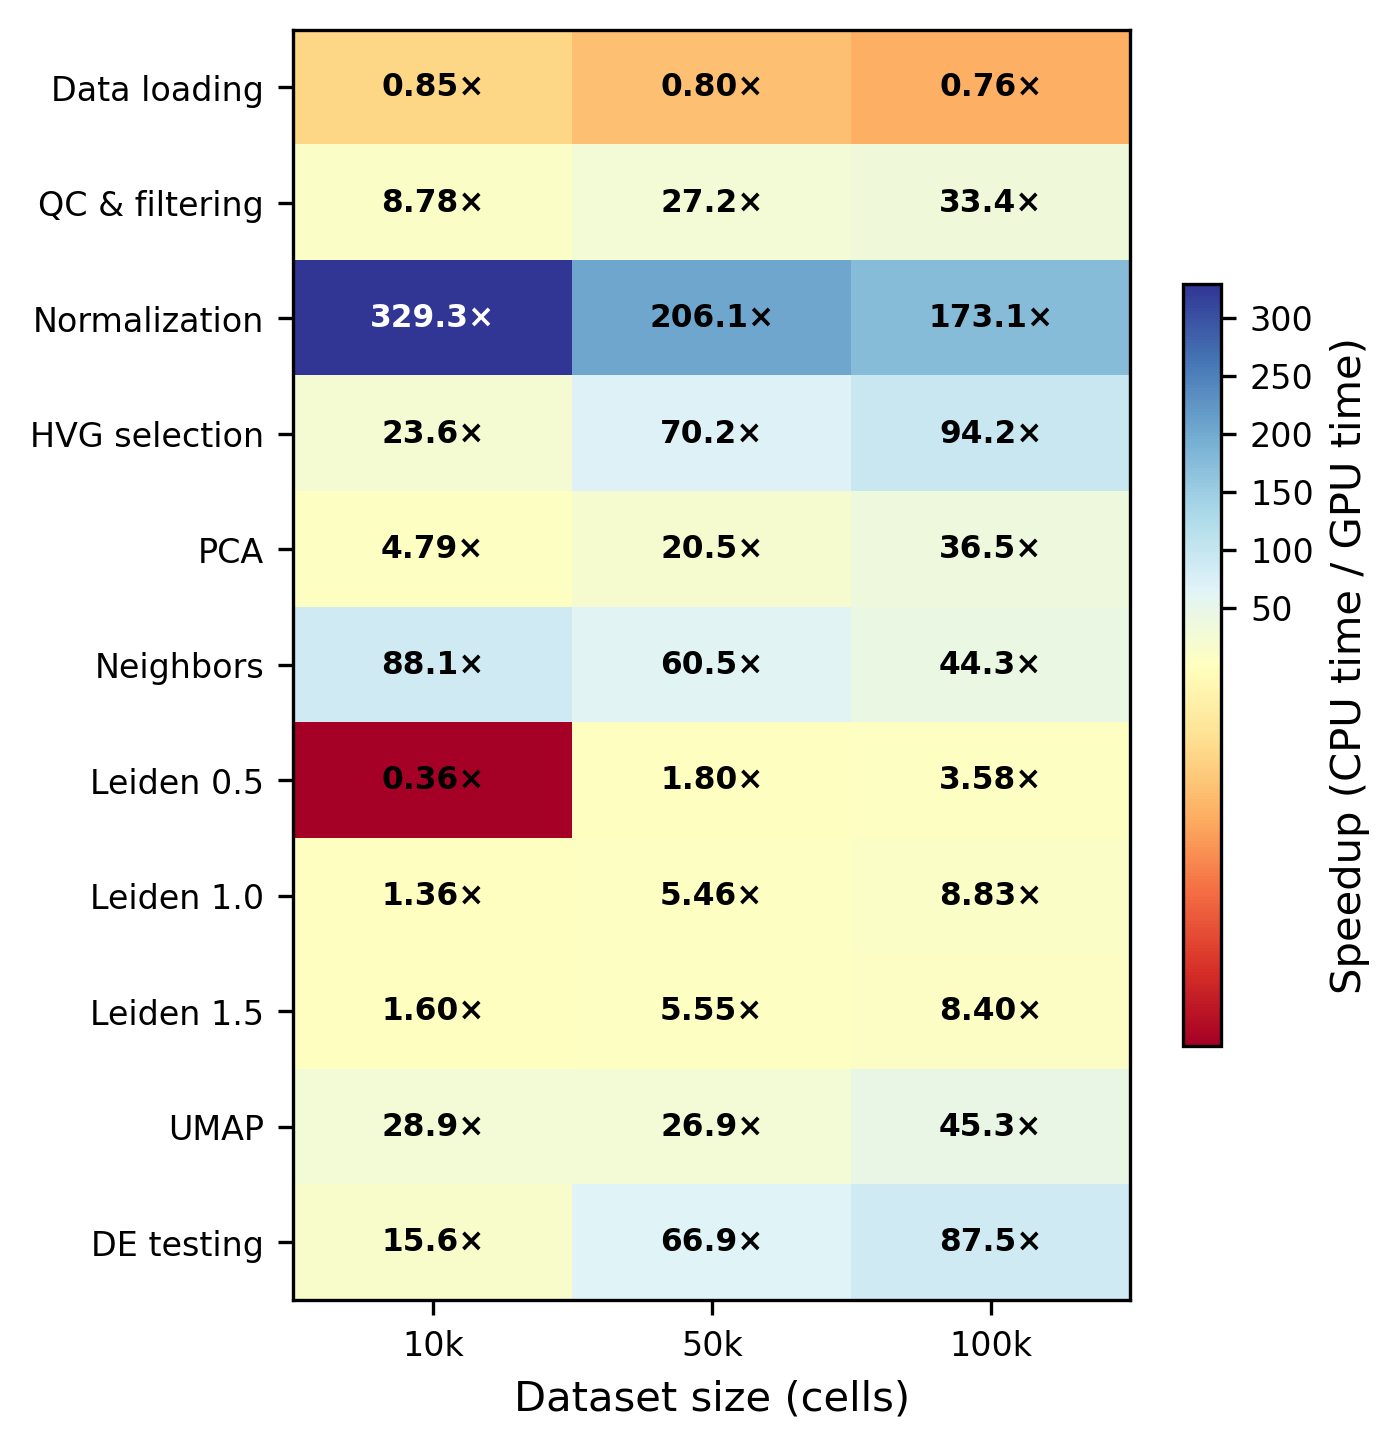
\includegraphics[width=0.85\textwidth,keepaspectratio,alt={Figure 1. Per-step speedup of single-GPU rapids-singlecell (1xH100 80 GB) relative to CPU Scanpy (100 cores) at 10k, 50k, and 100k cells. Values \textgreater{} 1 indicate GPU is faster. Normalisation achieves up to 329x speedup; data loading shows a modest CPU advantage (0.76-0.85x).}]{figures/fig1_speedup_heatmap.png}}
\caption{\textbf{Figure 1.} Per-step speedup of single-GPU
rapids-singlecell (1xH100 80 GB) relative to CPU Scanpy (100 cores) at
10k, 50k, and 100k cells. Values \textgreater{} 1 indicate GPU is
faster. Normalisation achieves up to 329x speedup; data loading shows a
modest CPU advantage (0.76-0.85x).}
\end{figure}

\begin{figure}
\centering
\pandocbounded{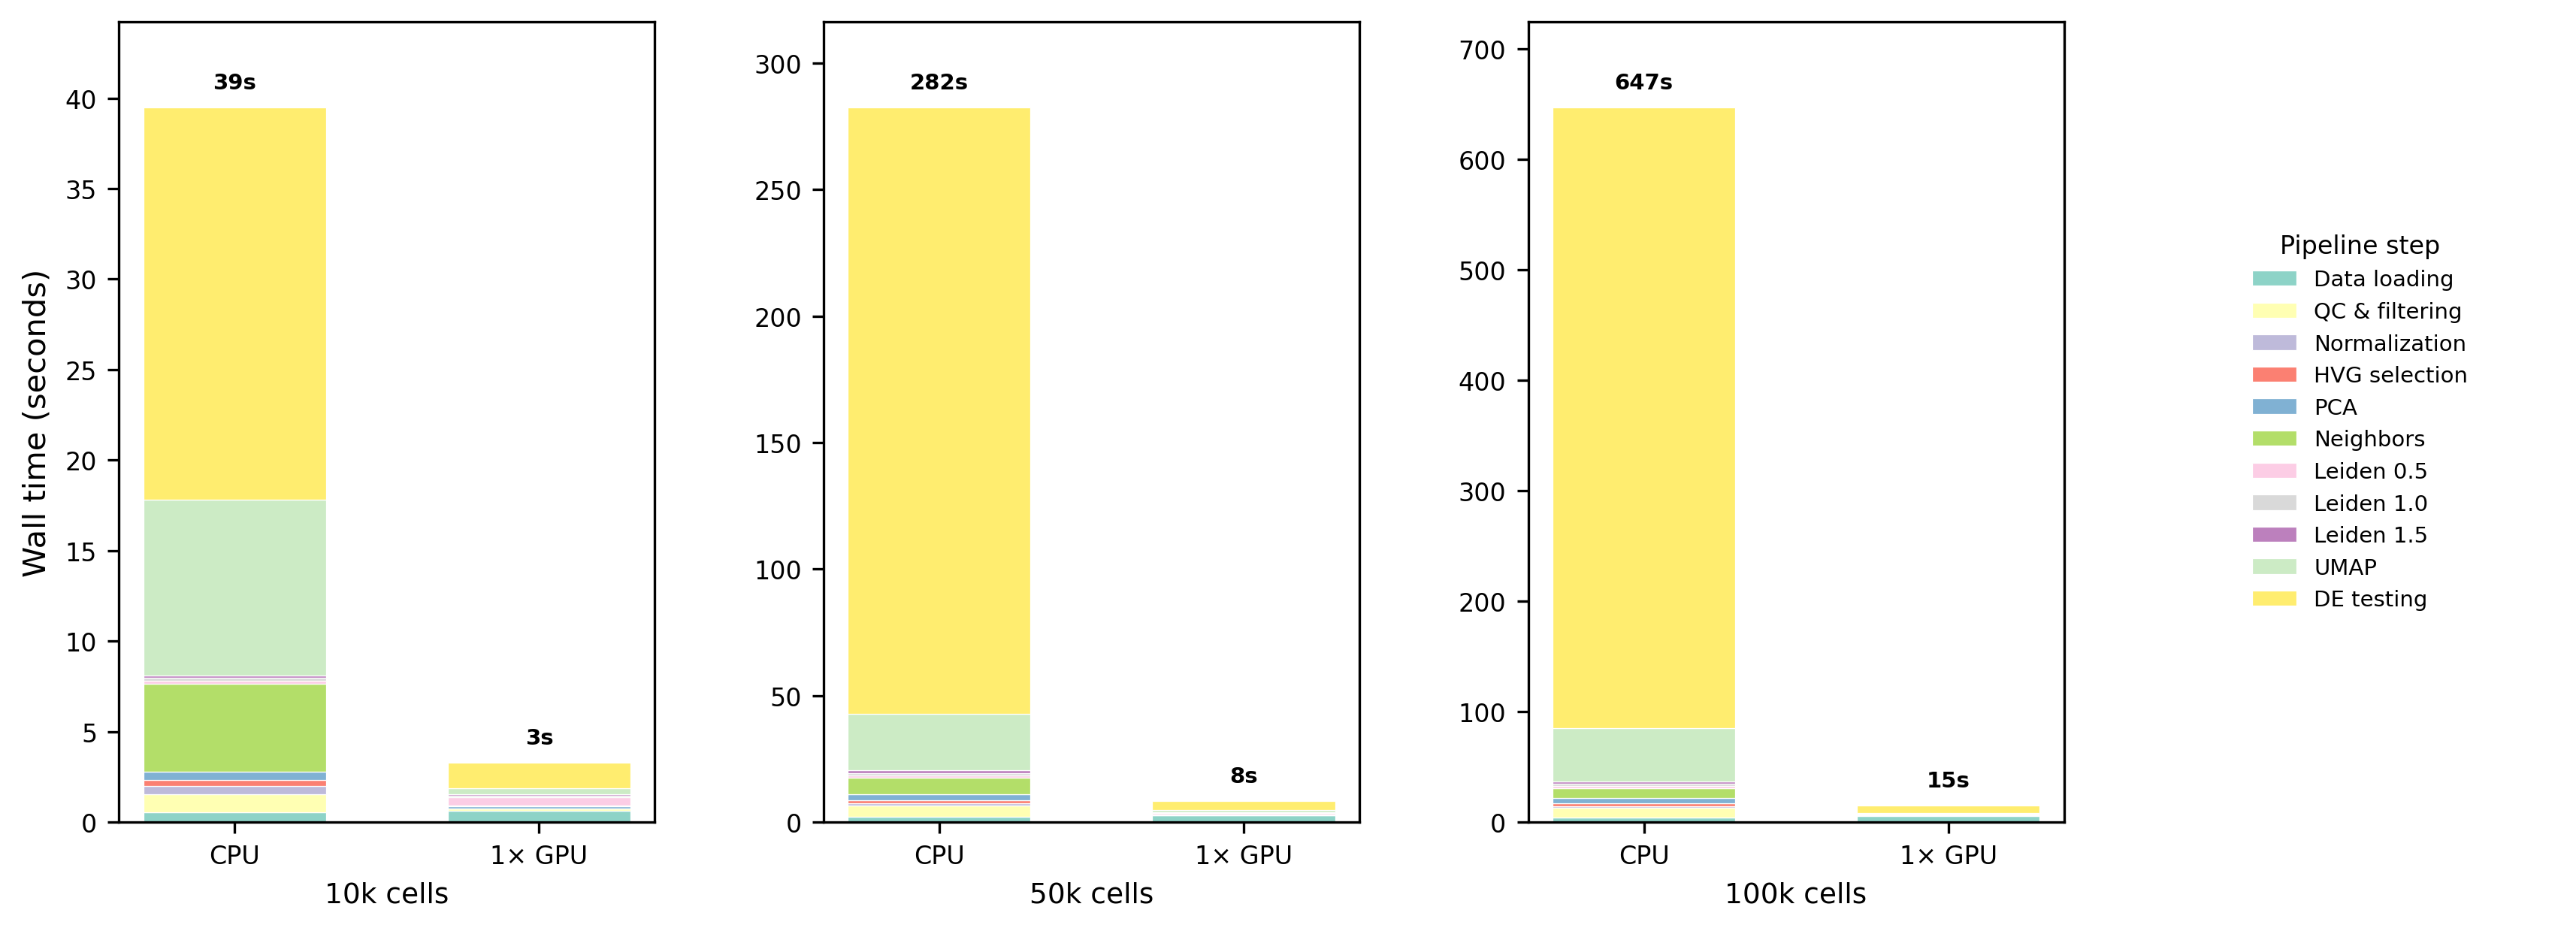
\includegraphics[width=0.85\textwidth,keepaspectratio,alt={Figure 2. Step-level wall time decomposition for CPU vs single-GPU at 10k, 50k, and 100k cells. On CPU, DE testing and neighbour graph construction dominate; on GPU, all steps complete in seconds.}]{figures/fig5_timing_breakdown.png}}
\caption{\textbf{Figure 2.} Step-level wall time decomposition for CPU
vs single-GPU at 10k, 50k, and 100k cells. On CPU, DE testing and
neighbour graph construction dominate; on GPU, all steps complete in
seconds.}
\end{figure}

However, not all operations benefited equally from GPU acceleration.
Data loading from disk was actually faster on CPU across all scales
(0.76-0.85x GPU/CPU), because the fixed overhead of CUDA context
initialisation and RMM pool allocation dominated the short data transfer
itself: PCIe Gen5 bandwidth (128 GB/s) is not saturated at these
sub-gigabyte dataset sizes, and the transfer completes in milliseconds.
We note that our pipeline relies on \texttt{h5py}-based readers that
route data through CPU RAM, precluding GPU Direct Storage (GDS)
optimisations that would bypass the CPU entirely; this remains an avenue
for future improvement. Similarly, Leiden clustering showed a clear
dependence on problem size: at 10k cells, CPU was faster (0.36x) due to
cuGraph's higher constant-time overhead for graph partitioning
operations on small graphs, but GPU performance improved substantially
as the graph size increased, with GPU overtaking CPU at 50k cells (1.80x
speedup) and achieving 3.58x speedup at 100k cells.

\subsubsection{Multi-GPU scaling is sublinear: CPU preprocessing
dominates}\label{multi-gpu-scaling-is-sublinear-cpu-preprocessing-dominates}

Adding GPUs beyond two provided diminishing returns (Fig. 3). At 500k
cells, wall time was virtually identical for 2, 4, and 8 GPUs (124.5,
125.0, and 124.6 s, respectively). At 1.3M cells, 8 GPUs (435.2 s) were
only 12\% faster than 2 GPUs (493.3 s).

The timing breakdown (Fig. 4) reveals why: in a representative 8-GPU run
at 1.3M cells (total 463.4 s), CPU preprocessing (data loading + QC +
normalisation + HVG selection) consumed 348.7 s (75\%), the multi-GPU
phase (PCA + neighbours) took only 17.5 s (4\%), and single-GPU
operations (transfer + scale + Leiden + UMAP + DE) took 97.2 s (21\%).
Since CPU preprocessing is constant regardless of GPU count, and
Leiden/UMAP/DE execute on a single GPU, only the PCA and neighbour steps
benefit from additional GPUs, a classic instance of Amdahl's law
\citep{Amdahl1967}.

\begin{figure}
\centering
\pandocbounded{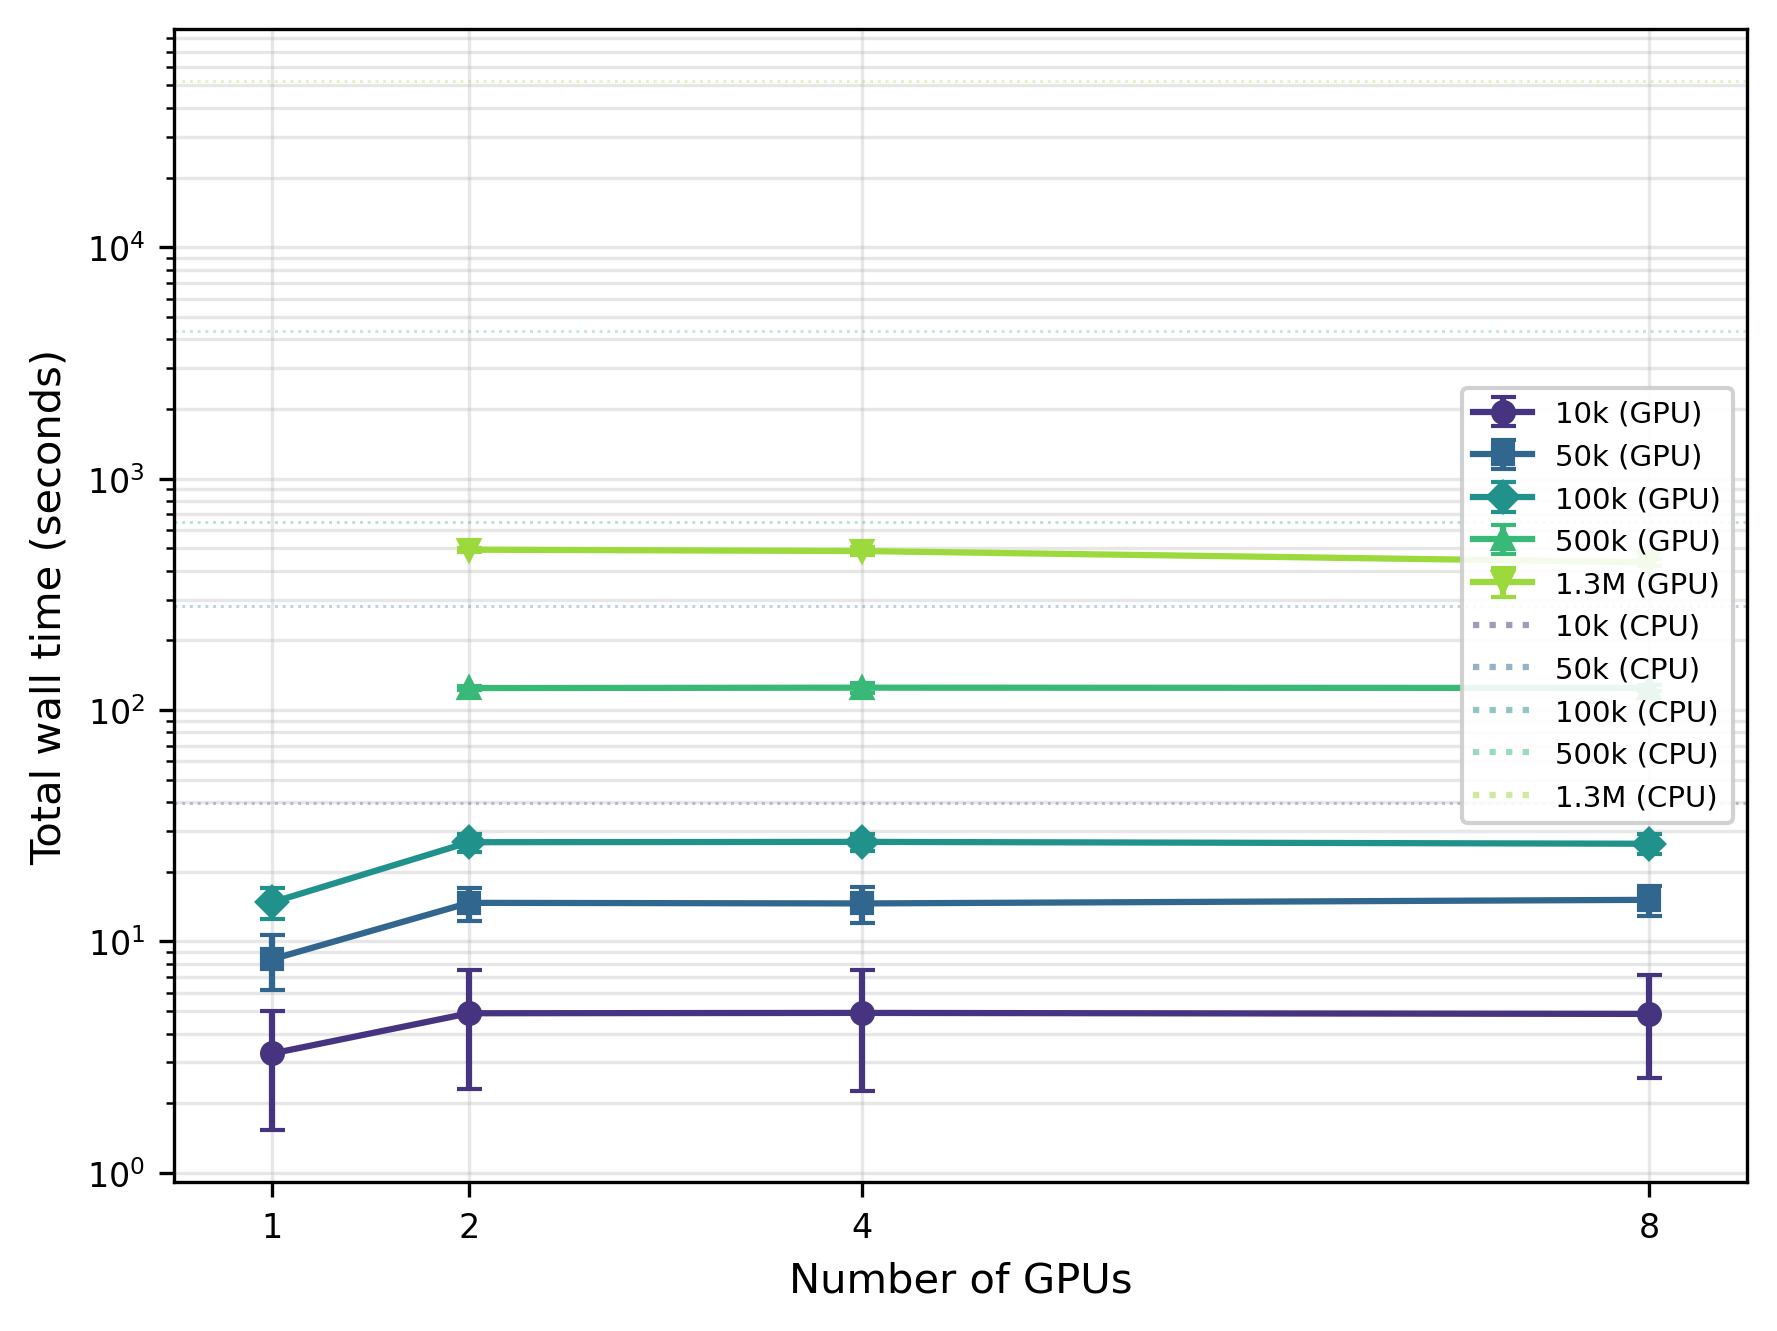
\includegraphics[width=0.85\textwidth,keepaspectratio,alt={Figure 3. Total pipeline wall time vs number of GPUs (1, 2, 4, 8 H100), one line per dataset size. Error bars: SD over five repeats. Horizontal dotted lines: CPU baselines. Logarithmic y-axis. Flat GPU curves demonstrate sublinear multi-GPU scaling.}]{figures/fig2_scaling_plot.png}}
\caption{\textbf{Figure 3.} Total pipeline wall time vs number of GPUs
(1, 2, 4, 8 H100), one line per dataset size. Error bars: SD over five
repeats. Horizontal dotted lines: CPU baselines. Logarithmic y-axis.
Flat GPU curves demonstrate sublinear multi-GPU scaling.}
\end{figure}

\begin{figure}
\centering
\pandocbounded{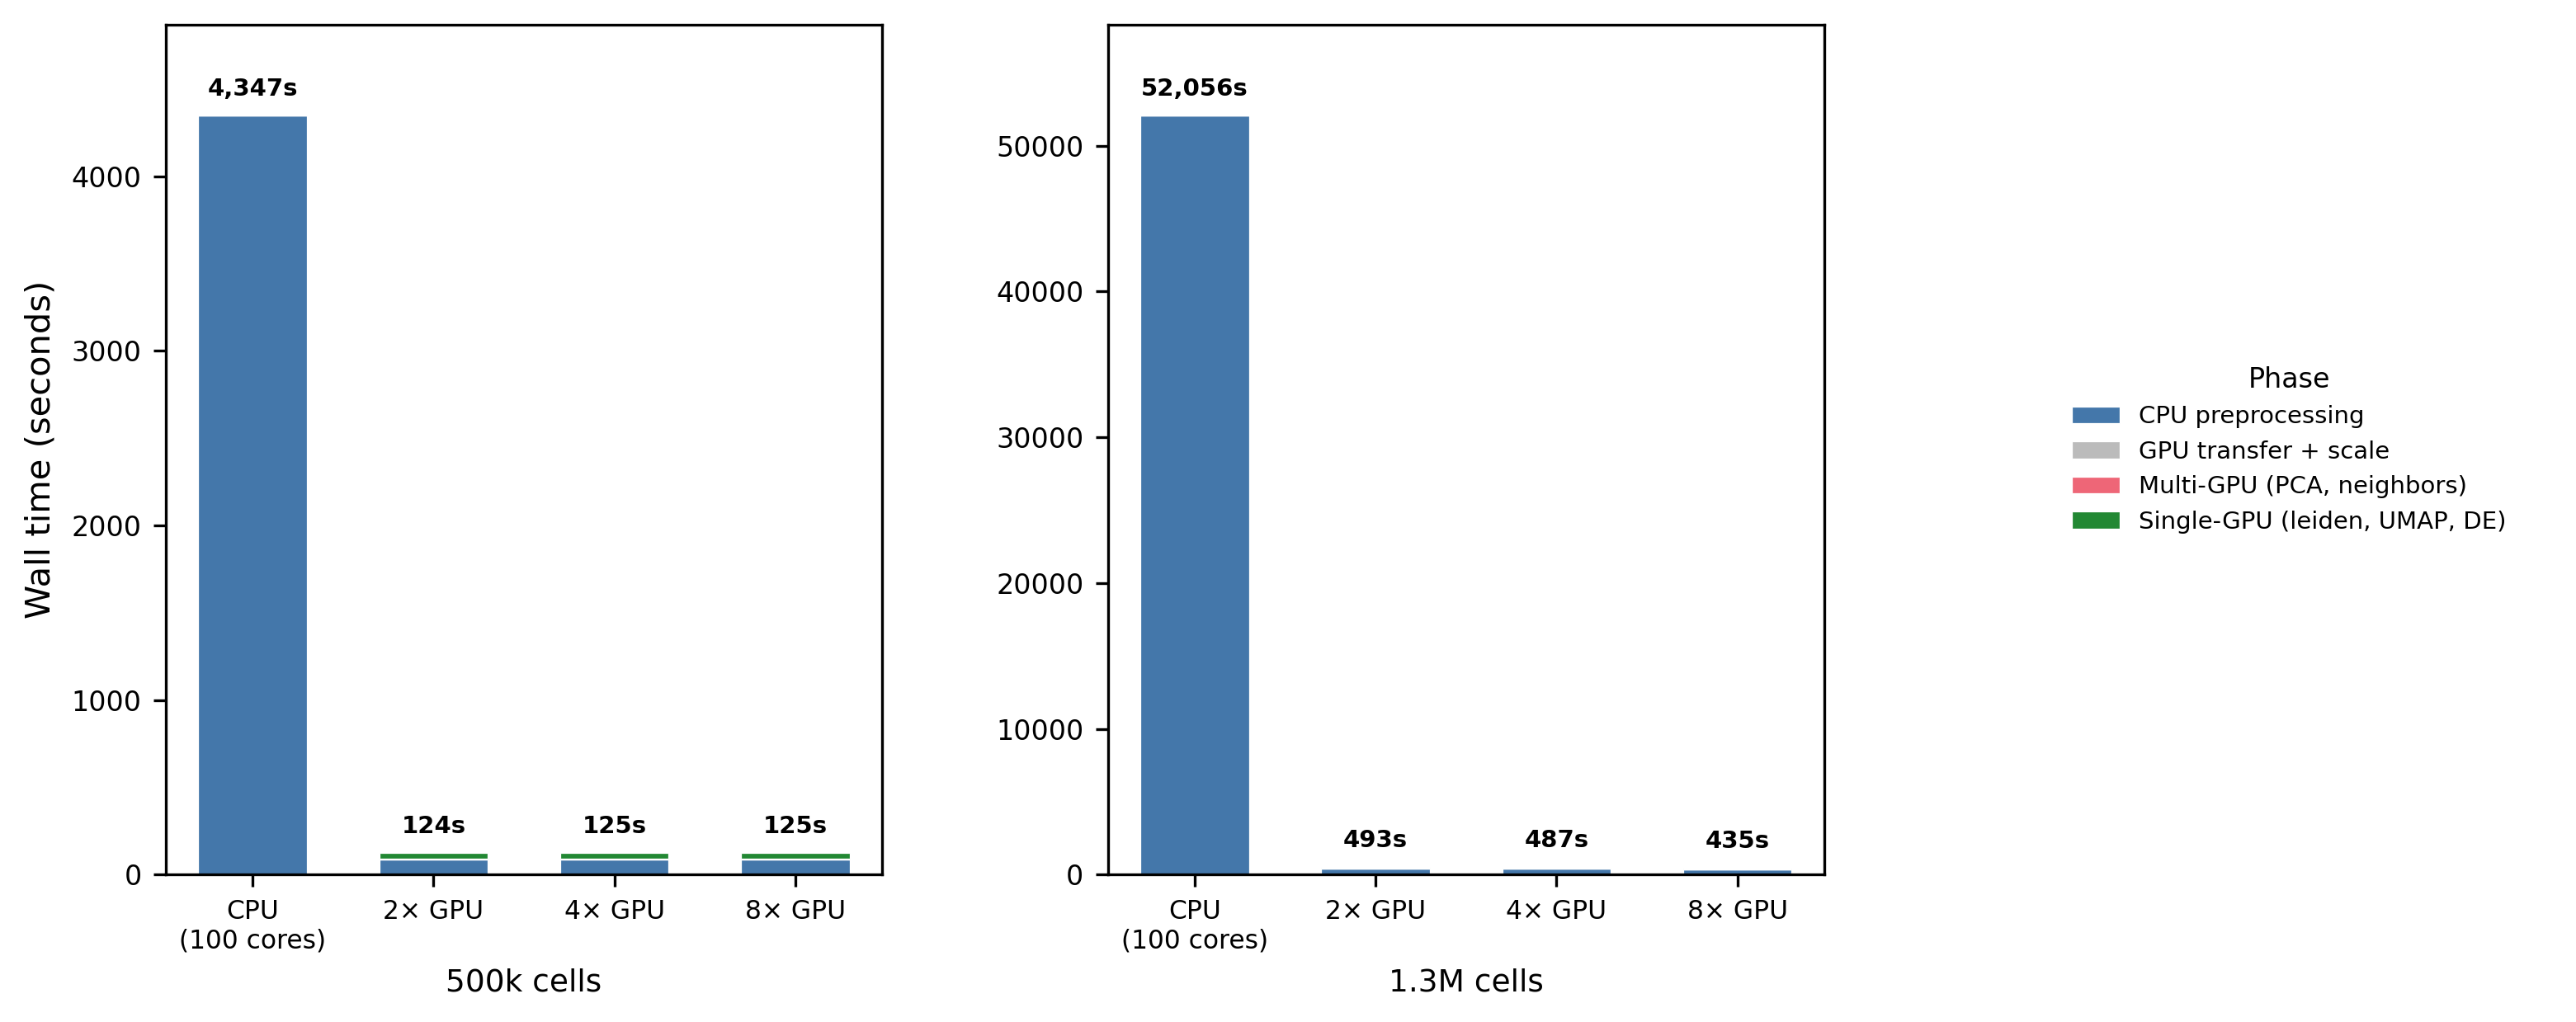
\includegraphics[width=0.85\textwidth,keepaspectratio,alt={Figure 4. Multi-GPU hybrid pipeline breakdown at 500k and 1.3M cells. CPU preprocessing (blue) dominates wall time; the multi-GPU phase (PCA + neighbours, pink) is a small fraction, explaining flat multi-GPU scaling.}]{figures/fig6_multigpu_breakdown.png}}
\caption{\textbf{Figure 4.} Multi-GPU hybrid pipeline breakdown at 500k
and 1.3M cells. CPU preprocessing (blue) dominates wall time; the
multi-GPU phase (PCA + neighbours, pink) is a small fraction, explaining
flat multi-GPU scaling.}
\end{figure}

\subsubsection{CPU and GPU produce biologically concordant
results}\label{cpu-and-gpu-produce-biologically-concordant-results}

Concordance analysis on the 10,000-cell dataset (Fig. 5) demonstrated
that the two pipelines yield near-identical biological conclusions,
despite computing on different processors and hardware. Upstream
analysis steps showed deterministic agreement: HVG selection was
perfectly concordant with all 2,000 genes identical between CPU and GPU
(Jaccard = 1.000), and PCA loadings were perfectly correlated with mean
absolute Spearman rho = 1.000 across all 10 inspected principal
components. Neighbourhood graph construction achieved high overlap with
mean Jaccard = 0.930 (median = 0.938), though some variation in the
k-nearest neighbours across the graph was expected due to floating-point
precision differences.

Clustering concordance showed expected variations due to algorithm
stochasticity. Leiden clustering at different resolutions yielded
adjusted Rand indices ranging from 0.908 (resolution 1.0) to 0.963
(resolution 1.5), with corresponding normalised mutual information
values from 0.951 to 0.971. The slightly lower concordance at resolution
1.0, where both pipelines identified 40 clusters, reflects the inherent
stochasticity of the Leiden algorithm and minor differences in the
underlying graph-partitioning implementations provided by cuGraph (GPU)
versus igraph (CPU), rather than indicating any systematic bias. The
downstream biological results also aligned well: differential expression
log-fold-changes across 40 matched cluster pairs showed mean Spearman
correlation of 0.946, with 30 of the 40 pairs exceeding the stringent
threshold of rho \textgreater{} 0.97.

These concordance levels are consistent with the range of inter-method
variation reported in mixture-control benchmarks of scRNA-seq analysis
pipelines \citep{Tian2019} and systematic evaluations of clustering
algorithm variability \citep{Duo2020}, and support the conclusion that
GPU and CPU pipelines are interchangeable for biological interpretation.

\begin{figure}
\centering
\pandocbounded{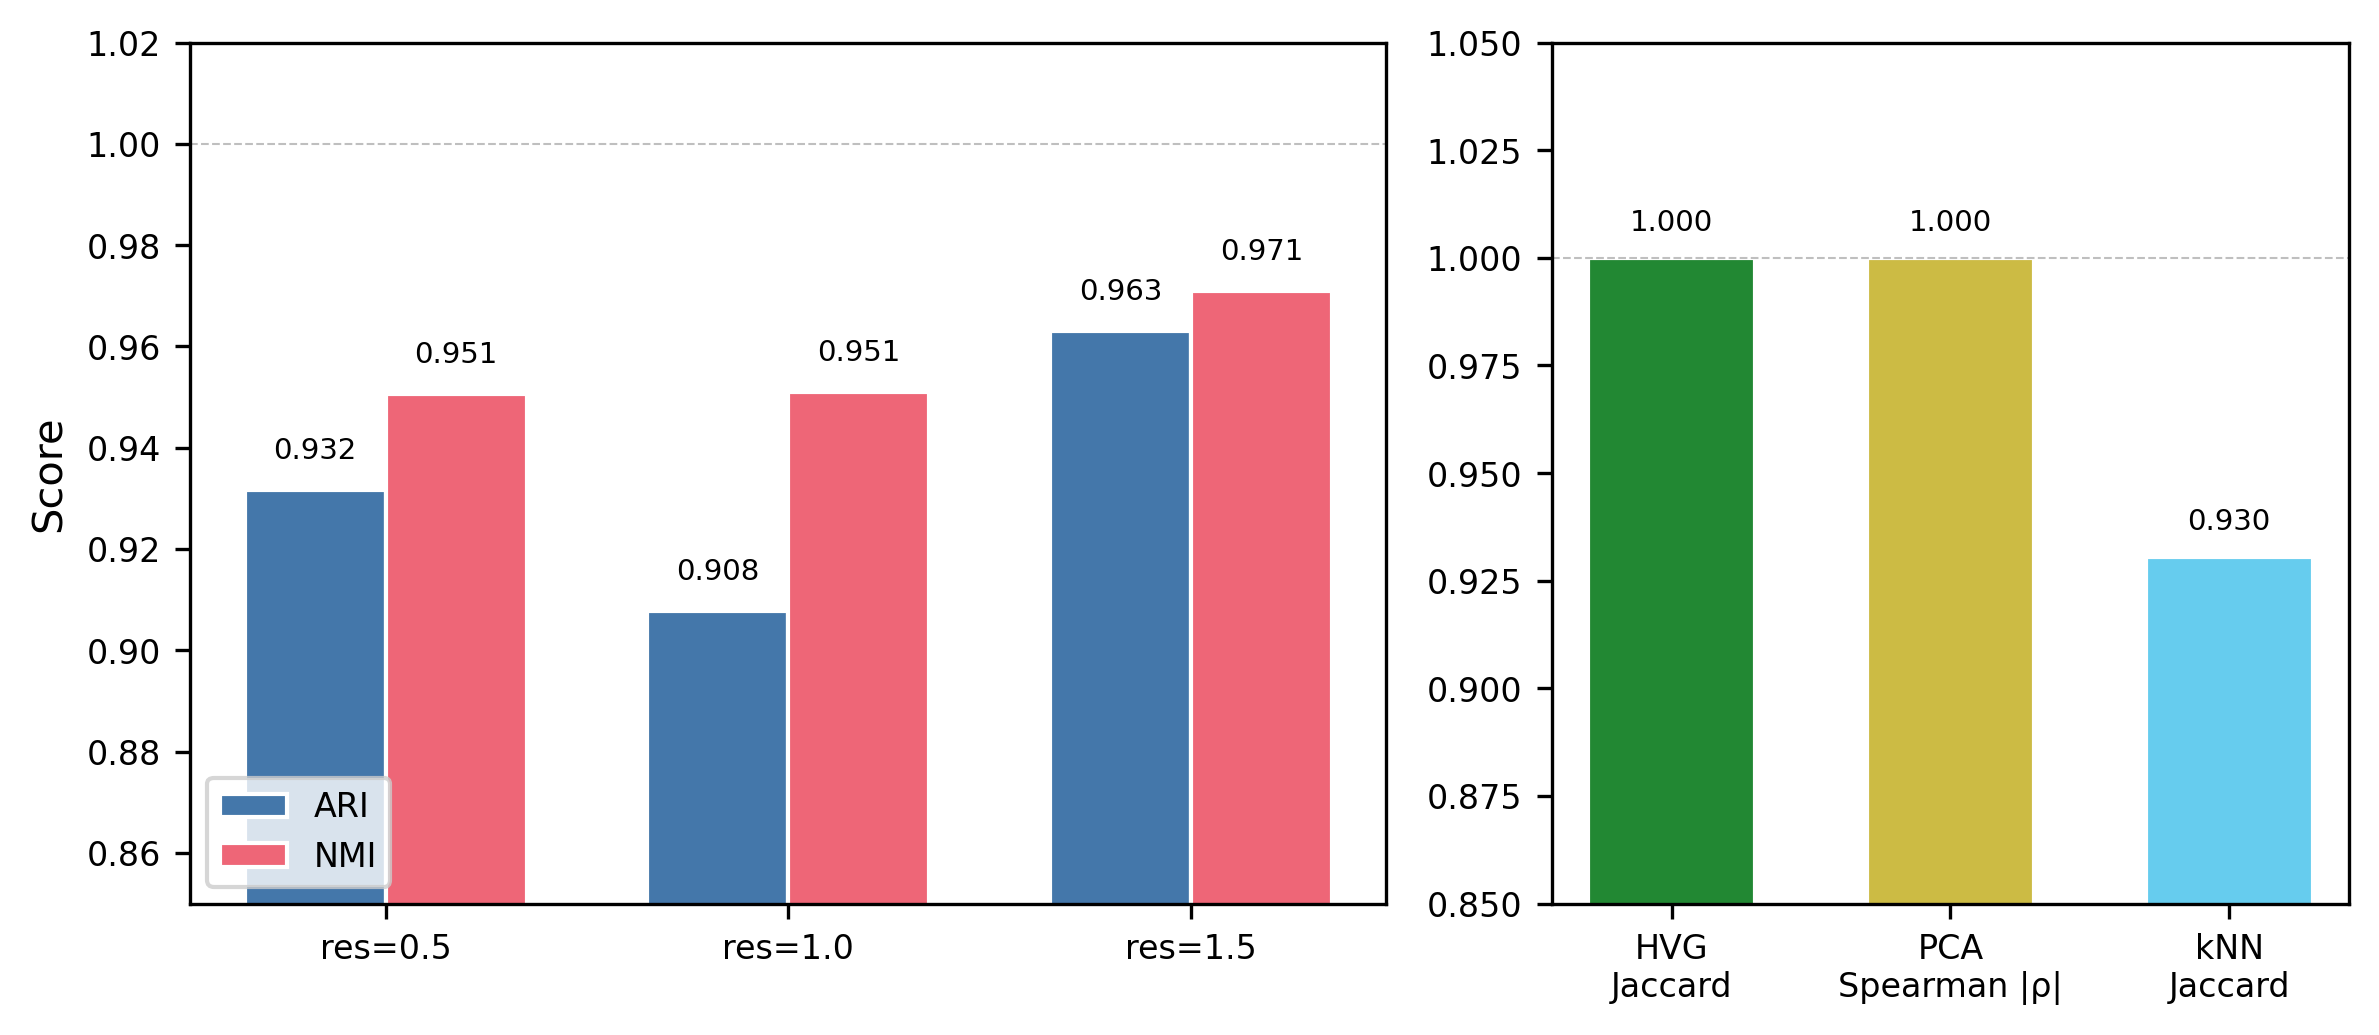
\includegraphics[width=0.85\textwidth,keepaspectratio,alt={Figure 5. Concordance between CPU and GPU pipelines on 10,000 cells. Left: ARI and NMI for Leiden clustering at three resolutions. Right: HVG Jaccard (1.000), PCA Spearman \textbar rho\textbar{} (1.000), and kNN Jaccard (0.930). All metrics indicate near-identical biological outputs.}]{figures/fig3_concordance.png}}
\caption{\textbf{Figure 5.} Concordance between CPU and GPU pipelines on
10,000 cells. Left: ARI and NMI for Leiden clustering at three
resolutions. Right: HVG Jaccard (1.000), PCA Spearman
\textbar rho\textbar{} (1.000), and kNN Jaccard (0.930). All metrics
indicate near-identical biological outputs.}
\end{figure}

\subsubsection{Memory is not a bottleneck at benchmark
scale}\label{memory-is-not-a-bottleneck-at-benchmark-scale}

At the scales covered by the main benchmark (10k to 1.3M cells), neither
memory tier was saturated. CPU RAM usage scaled approximately linearly
with cell count, from 1.2 GB at 10k to 107.4 GB at 1.3M cells (Fig. 6,
left panel), well below 6\% of the 2 TB system memory. The dominant
in-memory objects at 1.3M cells were the dense float32 matrix created
during scaling (1.3M x 2,000 HVGs x 4 bytes approximately 10.4 GB) and
the sparse raw count matrix (1.3M x 39,182 genes). GPU VRAM for
single-GPU runs was approximately constant at 40.7 GB across dataset
sizes, dominated by the pre-allocated RMM pool. For multi-GPU runs,
aggregate VRAM scaled with worker count: at 1.3M cells with 8 GPUs, the
aggregate peak was 134.2 GB (mean 16.8 GB per device, 21\% of 80 GB
capacity), well below the per-device limit. At these scales, therefore,
end-to-end throughput is set by compute and I/O, not memory; CPU RAM
becomes the binding constraint only in the extreme stress-test regime
discussed in the next subsection.

To verify that distributed computation was actually occurring across all
workers (rather than silently collapsing onto a single GPU, as reported
for some Dask-CUDA configurations), two independent pieces of evidence
support the multi-GPU claim. First, the aggregate peak VRAM at 1.3M
cells with 8 GPUs (134.2 GB) exceeds the 80 GB capacity of any single
H100 device; this working set could not have fit on one GPU alone, so
data must have been distributed across at least two devices. Second, we
verified through direct scheduler queries
(\texttt{client.run\_on\_scheduler()}) that all requested workers were
in the \texttt{running} state throughout each benchmark, after
identifying and fixing a reporting bug in the client-side cache
(\texttt{client.scheduler\_info()}) that occasionally undercounted
active workers. Per-device VRAM traces (available in the benchmark
result JSON files in the code repository) show balanced usage across
workers during the PCA and neighbour phases and fall back to a
single-GPU footprint only during Leiden and UMAP, which are implemented
as single-GPU operations in cuGraph 26.2.

\begin{figure}
\centering
\pandocbounded{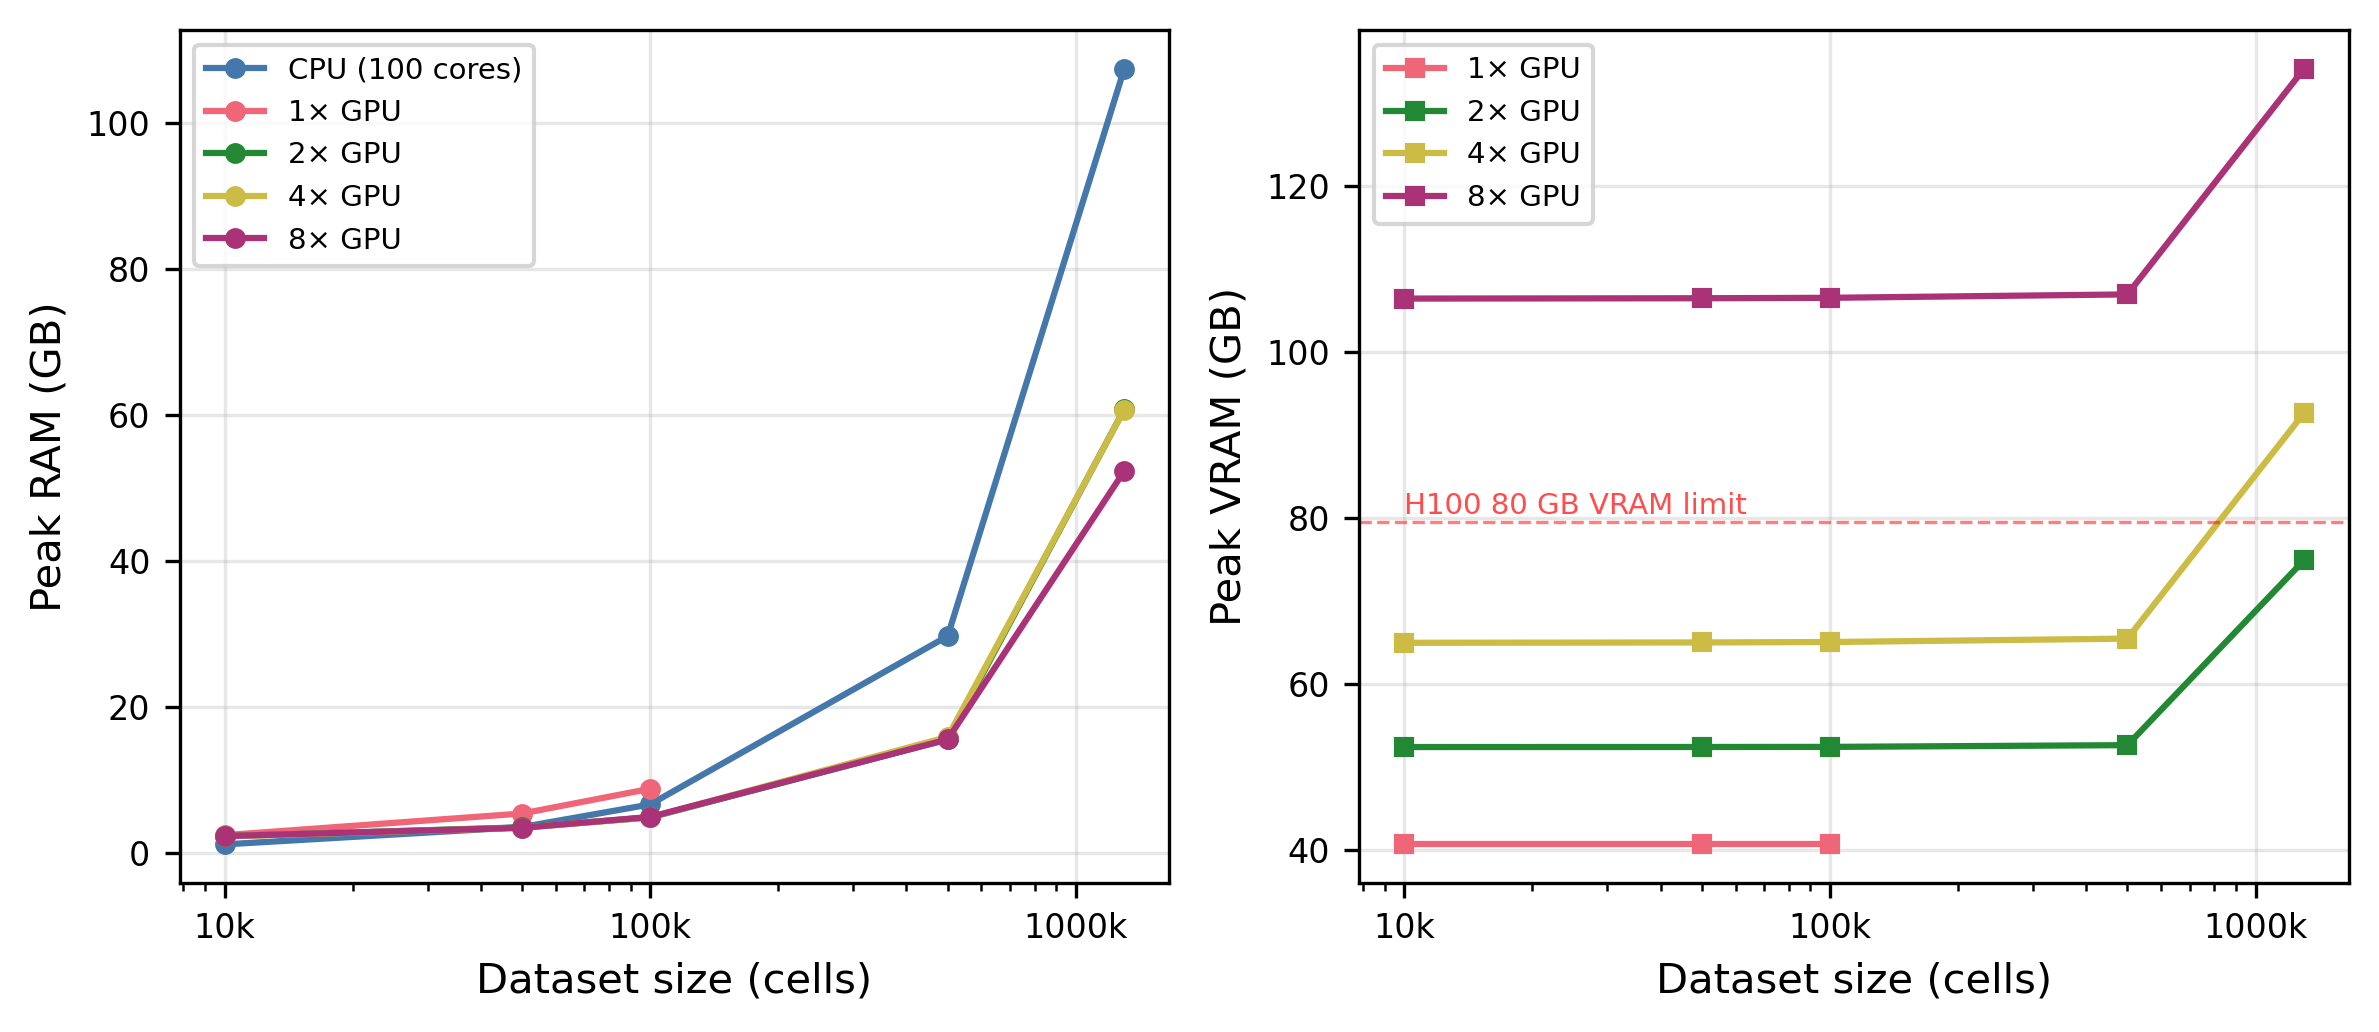
\includegraphics[width=0.85\textwidth,keepaspectratio,alt={Figure 6. Peak memory usage across dataset sizes. Left: CPU RAM; right: GPU VRAM (per-device maximum). Dashed red line: H100 80 GB VRAM limit. CPU RAM grows super-linearly; GPU VRAM is approximately constant for single-GPU runs due to RMM pool pre-allocation.}]{figures/fig4_memory_profile.png}}
\caption{\textbf{Figure 6.} Peak memory usage across dataset sizes.
Left: CPU RAM; right: GPU VRAM (per-device maximum). Dashed red line:
H100 80 GB VRAM limit. CPU RAM grows super-linearly; GPU VRAM is
approximately constant for single-GPU runs due to RMM pool
pre-allocation.}
\end{figure}

\subsubsection{Stress test: 11.9 million cells on one DGX H100
node}\label{stress-test-11.9-million-cells-on-one-dgx-h100-node}

To locate the true capacity limit of the DGX H100 node, we ran a
separate stress test with the \emph{memory-optimised pipeline} described
in Methods (Section ``Stress test: maximum capacity''). This variant
moves scaling to CPU (exploiting the 2 TB system RAM), distributes PCA
across all 8 GPUs via a covariance-matrix method, and replaces the full
data matrix on GPU with an empty sparse placeholder after PCA so that
only the low-dimensional embedding (n x 50 floats) resides on any GPU.

A binary search for the maximum processable cell count (Table 5) showed
that the pipeline succeeded at 11.9 million cells (119 min) and failed
at 12.0 million cells (Leiden out-of-memory, SLURM signal 9). A separate
test at 13.7 million cells failed earlier, during the CPU-side
sparse-to-dense scaling step.

The failure point is counter-intuitive at first reading: the stable peak
RAM at 11.9M was 535 GB (26\% of the 2 TB machine, 30\% of the 1.8 TB
SLURM job allocation), leaving apparent headroom. Stable peak aggregate
VRAM was only 49 GB out of 640 GB (7.6\%). Neither of these stable
figures alone explains why 12M cells fails. The actual capacity limit is
imposed by \textbf{transient memory peaks during individual
preprocessing operations}: spikes that briefly multiply the stable
footprint and that \texttt{psutil} samples only sporadically (Table 6).
The combined working set during Leiden graph construction at 12M nodes
exceeds the 1.8 TB SLURM allocation, triggering cgroup SIGKILL. The
13.7M failure is a distinct transient spike during sparse-to-dense
scaling that saturates memory even earlier.

We also tested cuML KMeans as a GPU-native clustering alternative to
Leiden, but the failure point was identical (13.7M) because the
out-of-memory event occurred during CPU preprocessing, before clustering
was invoked. Similarly, a sparse-scatter optimisation that avoided the
CPU-side dense matrix was tested at 14M cells but failed during Scanpy's
HVG selection step, confirming that Scanpy's CPU-side preprocessing is
the ultimate capacity bottleneck.

Inspired by the chunked-preprocessing strategy of ScaleSC
\citep{Hu2025}, we also implemented a third variant that performs HVG
selection on per-gene running statistics accumulated over 100,000-cell
batches and computes PCA via batch-wise covariance accumulation, both
directly from the sparse matrix without ever materialising a dense
intermediate on CPU. This variant succeeded at 12.0 million cells (862
GB peak RAM, 10 GB aggregate VRAM, 156 min) but failed at 15.0 million
cells during the CSR-to-CSC layout conversion required for HVG column
slicing.

\begin{longtable}[]{@{}
  >{\raggedleft\arraybackslash}p{(\linewidth - 10\tabcolsep) * \real{0.0986}}
  >{\raggedleft\arraybackslash}p{(\linewidth - 10\tabcolsep) * \real{0.2113}}
  >{\raggedleft\arraybackslash}p{(\linewidth - 10\tabcolsep) * \real{0.1972}}
  >{\raggedleft\arraybackslash}p{(\linewidth - 10\tabcolsep) * \real{0.2113}}
  >{\raggedright\arraybackslash}p{(\linewidth - 10\tabcolsep) * \real{0.1690}}
  >{\raggedright\arraybackslash}p{(\linewidth - 10\tabcolsep) * \real{0.1127}}@{}}
\caption{\textbf{Table 5.} Stress test results: maximum cell count on a
single DGX H100 node (8xH100, 2 TB RAM) using the memory-optimised
pipeline. Timings exclude DE testing, which was benchmarked separately
(Table 7).}\label{tbl:stress}\tabularnewline
\toprule\noalign{}
\begin{minipage}[b]{\linewidth}\raggedleft
Cells
\end{minipage} & \begin{minipage}[b]{\linewidth}\raggedleft
Runtime (min)
\end{minipage} & \begin{minipage}[b]{\linewidth}\raggedleft
CPU RAM (GB)
\end{minipage} & \begin{minipage}[b]{\linewidth}\raggedleft
GPU VRAM (GB)
\end{minipage} & \begin{minipage}[b]{\linewidth}\raggedright
Clustering
\end{minipage} & \begin{minipage}[b]{\linewidth}\raggedright
Status
\end{minipage} \\
\midrule\noalign{}
\endfirsthead
\toprule\noalign{}
\begin{minipage}[b]{\linewidth}\raggedleft
Cells
\end{minipage} & \begin{minipage}[b]{\linewidth}\raggedleft
Runtime (min)
\end{minipage} & \begin{minipage}[b]{\linewidth}\raggedleft
CPU RAM (GB)
\end{minipage} & \begin{minipage}[b]{\linewidth}\raggedleft
GPU VRAM (GB)
\end{minipage} & \begin{minipage}[b]{\linewidth}\raggedright
Clustering
\end{minipage} & \begin{minipage}[b]{\linewidth}\raggedright
Status
\end{minipage} \\
\midrule\noalign{}
\endhead
\bottomrule\noalign{}
\endlastfoot
3.4M & 18 & 155 & 49 & KMeans & Pass \\
6.9M & 38 & 308 & 49 & KMeans & Pass \\
10.3M & 92 & 465 & 49 & KMeans & Pass \\
11.5M & 114 & 517 & 49 & Leiden & Pass \\
11.9M & 119 & 535 & 49 & Leiden & \textbf{Pass (max)} \\
12.0M & --- & --- & --- & Leiden & Fail (Leiden OOM) \\
13.7M & --- & --- & --- & Leiden & Fail (scale OOM) \\
\end{longtable}

The three smaller rows were benchmarked with cuML KMeans rather than
Leiden to isolate the CPU preprocessing cost from the clustering cost;
KMeans and Leiden exhibit the same CPU-RAM and CPU-preprocessing
footprint in this pipeline (see Section ``Stress test: maximum
capacity'') and the failure point at scale is identical (13.7M, CPU-side
scale step), so the KMeans rows are included here as valid ascending
points on the runtime/memory curves.

\begin{longtable}[]{@{}
  >{\raggedright\arraybackslash}p{(\linewidth - 2\tabcolsep) * \real{0.8710}}
  >{\raggedleft\arraybackslash}p{(\linewidth - 2\tabcolsep) * \real{0.1290}}@{}}
\caption{\textbf{Table 6.} Memory budget at the 12M-cell failure point,
showing why the stable 535 GB baseline translates to an out-of-memory
event. Baseline values are measured (the 535 GB subtotal matches the
last successful run at 11.9M cells). Transient peak contributions are
estimated from operation-specific memory formulas and are not fully
captured by interval-based \protect\texttt{psutil} sampling; the
combined peak during Leiden is what exceeds the 1.8 TB SLURM allocation
and triggers OOM at 12M.}\label{tbl:memory_budget}\tabularnewline
\toprule\noalign{}
\begin{minipage}[b]{\linewidth}\raggedright
Memory usage at 12M cells
\end{minipage} & \begin{minipage}[b]{\linewidth}\raggedleft
GB
\end{minipage} \\
\midrule\noalign{}
\endfirsthead
\toprule\noalign{}
\begin{minipage}[b]{\linewidth}\raggedright
Memory usage at 12M cells
\end{minipage} & \begin{minipage}[b]{\linewidth}\raggedleft
GB
\end{minipage} \\
\midrule\noalign{}
\endhead
\bottomrule\noalign{}
\endlastfoot
\textbf{Baseline (stable peak, measured at 11.9M)} & \\
~~~~Sparse raw matrix \texttt{adata.X} (CSR, \textasciitilde5\% density)
& \textasciitilde190 \\
~~~~Sparse raw copy \texttt{adata.raw} (DE backup) &
\textasciitilde190 \\
~~~~Dense scaled HVG matrix (12M x 2,000, float32) & 96 \\
~~~~Scanpy metadata + Python runtime + allocator overhead &
\textasciitilde60 \\
~~~~\emph{Measured subtotal (11.9M, stable)} & \textbf{535} \\
\textbf{Transient peaks during individual operations} & \\
~~~~CSR to CSC layout conversion & +190 \\
~~~~Sparse to dense scaling (\texttt{sc.pp.scale}) & +200 \\
~~~~\texttt{adata.raw\ =\ adata.copy()} & +400 \\
~~~~Leiden graph construction (igraph + partitions at 12M nodes, k=15) &
+700 to 1,000 \\
~~~~\emph{Estimated combined peak during Leiden} &
\textbf{\textasciitilde1,500} \\
SLURM job allocation (\texttt{\#SBATCH\ -\/-mem=1800G}) & 1,800 \\
Physical machine memory & 2,048 \\
\end{longtable}

\subsubsection{Differential expression: pseudo-bulk is fastest and most
correct}\label{differential-expression-pseudo-bulk-is-fastest-and-most-correct}

The factorial differential expression benchmark at 3.4 million cells
across 41,000 genes and 81 Leiden clusters (Table 7) revealed important
trade-offs between computational efficiency and statistical rigor. To
keep the table tractable we reported all wall times against a single CPU
denominator, the t-test (5,598 s): a CPU Wilcoxon baseline at this scale
was infeasible to measure (extrapolation from smaller subsamples places
it above four hours), and pseudo-bulk operates on a different sample
unit (donor x cluster pseudo-samples rather than individual cells), so
no strict within-method CPU-to-GPU ratio exists for it. Consequently,
the speedup column should be read as ``which approach finishes fastest
overall'', not as a within-method GPU acceleration factor; t-test and
Wilcoxon are distinct statistical tests with different computational
complexity, and any direct runtime comparison between them is
descriptive, not inferential.

\begin{longtable}[]{@{}llrrr@{}}
\caption{\textbf{Table 7.} Differential expression benchmark at 3.4M
cells x 41k genes x 81 Leiden clusters. Speedup is relative to CPU
t-test (5,598 s).}\label{tbl:de}\tabularnewline
\toprule\noalign{}
Method & Backend & GPUs & Time (s) & Speedup \\
\midrule\noalign{}
\endfirsthead
\toprule\noalign{}
Method & Backend & GPUs & Time (s) & Speedup \\
\midrule\noalign{}
\endhead
\bottomrule\noalign{}
\endlastfoot
t-test & CPU & 0 & 5,598 & 1.0x \\
Pseudo-bulk (Wilcoxon) & CPU (aggregated) & 0 & 128 & 43.7x \\
Wilcoxon (scatter) & GPU & 8 & 826 & 6.8x \\
Wilcoxon (chunk-stream) & GPU & 1 & 831 & 6.7x \\
t-test (scatter) & GPU & 8 & 1,656 & 3.4x \\
t-test (chunk-stream) & GPU & 1 & 1,650 & 3.4x \\
\end{longtable}

Pseudo-bulk aggregation emerged as the dominant strategy: aggregating
raw counts by donor and cluster reduced the analysis from 3.4 million
individual cells to a few hundred pseudo-samples per cluster, completing
in 128 seconds (2.1 minutes), a 43.7x speedup relative to the cell-level
CPU t-test baseline (5,598 s, 93 minutes). Among cell-level tests on
GPU, Wilcoxon (826 s) was faster than t-test (1,656 s), and multi-GPU
scatter (826 s for Wilcoxon) was essentially equivalent to single-GPU
chunk-and-stream (831 s).

\subsection{Spatial transcriptomics}\label{spatial-transcriptomics-1}

\subsubsection{GPU speedup scales dramatically with platform
resolution}\label{gpu-speedup-scales-dramatically-with-platform-resolution}

Table 8 summarises the spatial benchmark results across three Visium
platforms.

\begin{longtable}[]{@{}
  >{\raggedright\arraybackslash}p{(\linewidth - 12\tabcolsep) * \real{0.1111}}
  >{\raggedleft\arraybackslash}p{(\linewidth - 12\tabcolsep) * \real{0.1222}}
  >{\raggedleft\arraybackslash}p{(\linewidth - 12\tabcolsep) * \real{0.1778}}
  >{\raggedleft\arraybackslash}p{(\linewidth - 12\tabcolsep) * \real{0.1667}}
  >{\raggedleft\arraybackslash}p{(\linewidth - 12\tabcolsep) * \real{0.1000}}
  >{\raggedleft\arraybackslash}p{(\linewidth - 12\tabcolsep) * \real{0.1556}}
  >{\raggedleft\arraybackslash}p{(\linewidth - 12\tabcolsep) * \real{0.1667}}@{}}
\caption{\textbf{Table 8.} Spatial transcriptomics benchmark results
(RTX 4090, mean of repeats
2-5).}\label{tbl:spatial_summary}\tabularnewline
\toprule\noalign{}
\begin{minipage}[b]{\linewidth}\raggedright
Platform
\end{minipage} & \begin{minipage}[b]{\linewidth}\raggedleft
Spots/Bins
\end{minipage} & \begin{minipage}[b]{\linewidth}\raggedleft
CPU total (s)
\end{minipage} & \begin{minipage}[b]{\linewidth}\raggedleft
GPU total (s)
\end{minipage} & \begin{minipage}[b]{\linewidth}\raggedleft
Speedup
\end{minipage} & \begin{minipage}[b]{\linewidth}\raggedleft
CPU RAM (GB)
\end{minipage} & \begin{minipage}[b]{\linewidth}\raggedleft
GPU VRAM (GB)
\end{minipage} \\
\midrule\noalign{}
\endfirsthead
\toprule\noalign{}
\begin{minipage}[b]{\linewidth}\raggedright
Platform
\end{minipage} & \begin{minipage}[b]{\linewidth}\raggedleft
Spots/Bins
\end{minipage} & \begin{minipage}[b]{\linewidth}\raggedleft
CPU total (s)
\end{minipage} & \begin{minipage}[b]{\linewidth}\raggedleft
GPU total (s)
\end{minipage} & \begin{minipage}[b]{\linewidth}\raggedleft
Speedup
\end{minipage} & \begin{minipage}[b]{\linewidth}\raggedleft
CPU RAM (GB)
\end{minipage} & \begin{minipage}[b]{\linewidth}\raggedleft
GPU VRAM (GB)
\end{minipage} \\
\midrule\noalign{}
\endhead
\bottomrule\noalign{}
\endlastfoot
Visium v1 & 2,695 & 10.0 & 6.0 & 1.7x & 1.3 & 12.9 \\
Visium HD 8 um & 393,543 & 4,068 & 79 & 51.6x & 8.1 & 22.6 \\
Visium HD 2 um & 389,492 & 1,042 & 97 & 10.8x & 10.8 & 22.6 \\
\end{longtable}

End-to-end speedup increased from 1.7x on Visium v1 (2,695 spots) to
51.6x on Visium HD 8 um (393,543 bins) (Fig. 7), demonstrating that GPU
acceleration becomes increasingly valuable as spatial resolution
increases.

\begin{figure}
\centering
\pandocbounded{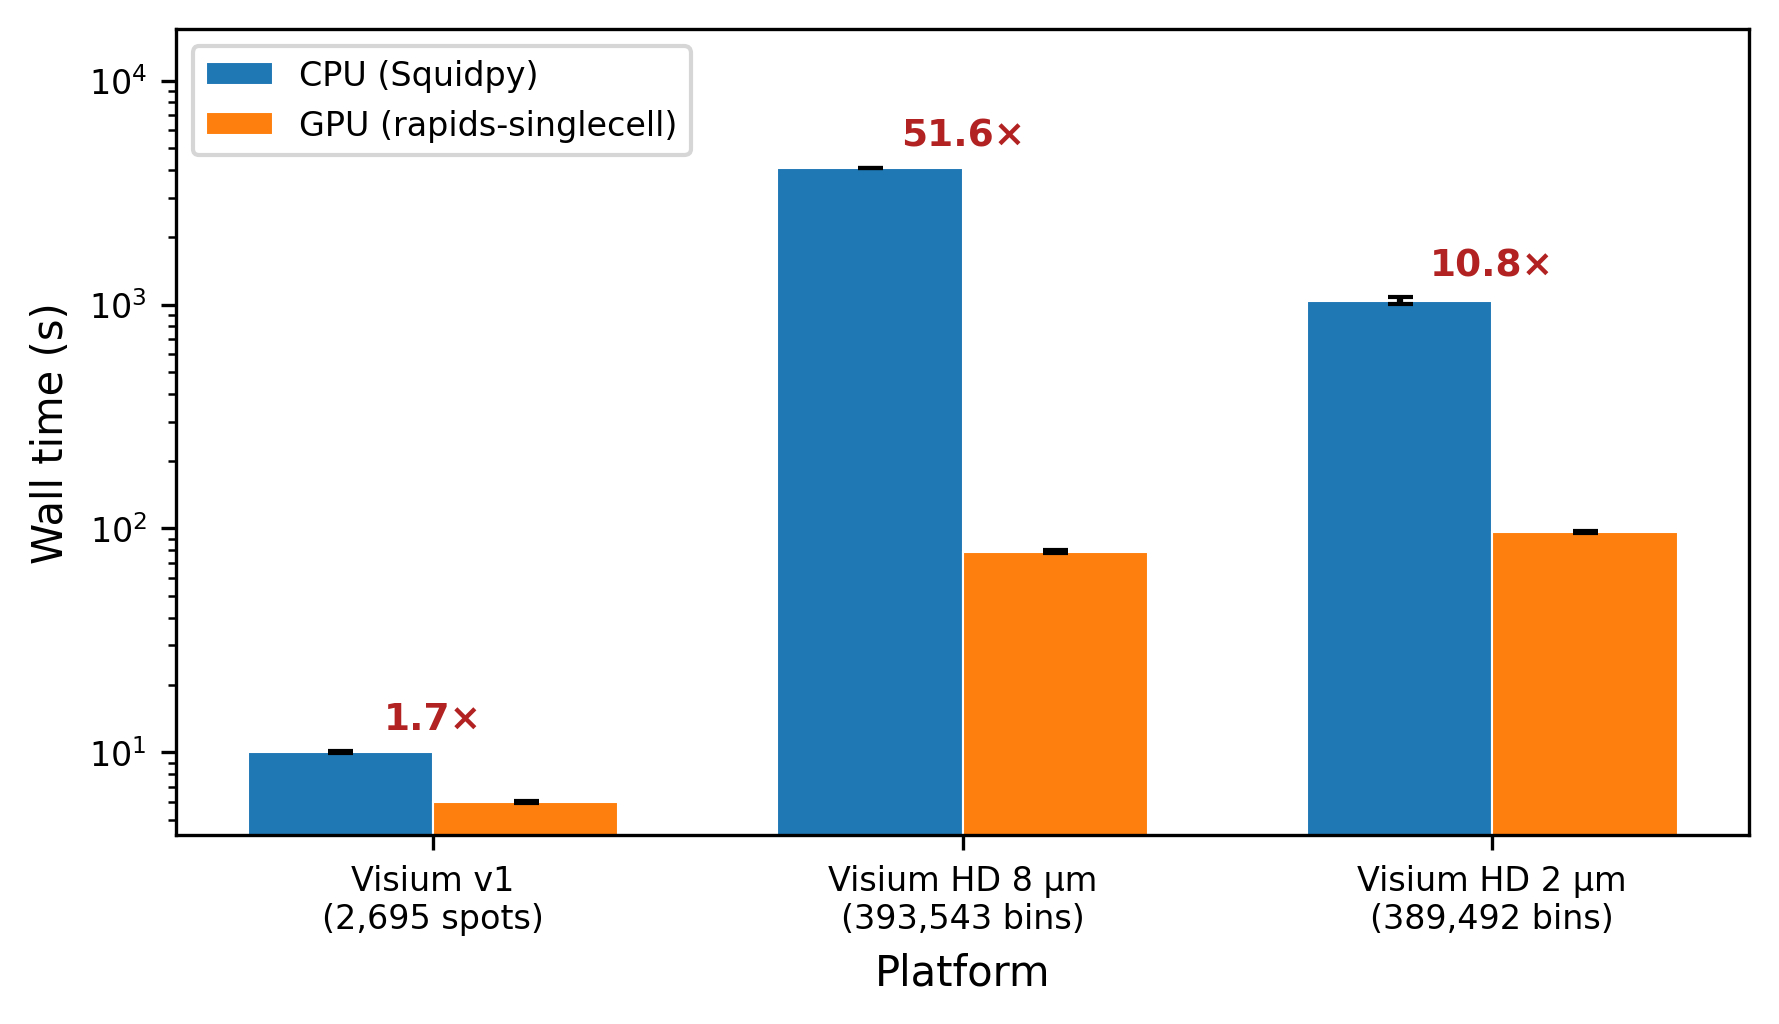
\includegraphics[width=0.85\textwidth,keepaspectratio,alt={Figure 7. Total pipeline wall time (CPU vs GPU) for three Visium spatial platforms on a single RTX 4090. End-to-end speedups range from 1.7x (Visium v1, 2,695 spots) to 51.6x (Visium HD 8 um, 393,543 bins). Error bars: standard deviation across repeats 2-5 (repeat 1 excluded for JIT warmup). HD 2 um was subsampled to 400k bins due to local VRAM constraints.}]{figures/fig7_spatial_speedup.png}}
\caption{\textbf{Figure 7.} Total pipeline wall time (CPU vs GPU) for
three Visium spatial platforms on a single RTX 4090. End-to-end speedups
range from 1.7x (Visium v1, 2,695 spots) to 51.6x (Visium HD 8 um,
393,543 bins). Error bars: standard deviation across repeats 2-5 (repeat
1 excluded for JIT warmup). HD 2 um was subsampled to 400k bins due to
local VRAM constraints.}
\end{figure}

The dominant contributor to the HD 8 um speedup was co-occurrence
analysis, which achieved a 3,272x speedup (from 3,573 s on CPU to 1.09 s
on GPU; Fig. 8). The CPU implementation computes pairwise cluster
co-occurrence across distance intervals with O(n\^{}2) complexity per
interval, while the GPU implementation parallelises this computation
across all bins and intervals simultaneously. At 393,543 bins with 7
Leiden clusters, co-occurrence alone consumed 88\% of the CPU pipeline
time.

\begin{figure}
\centering
\pandocbounded{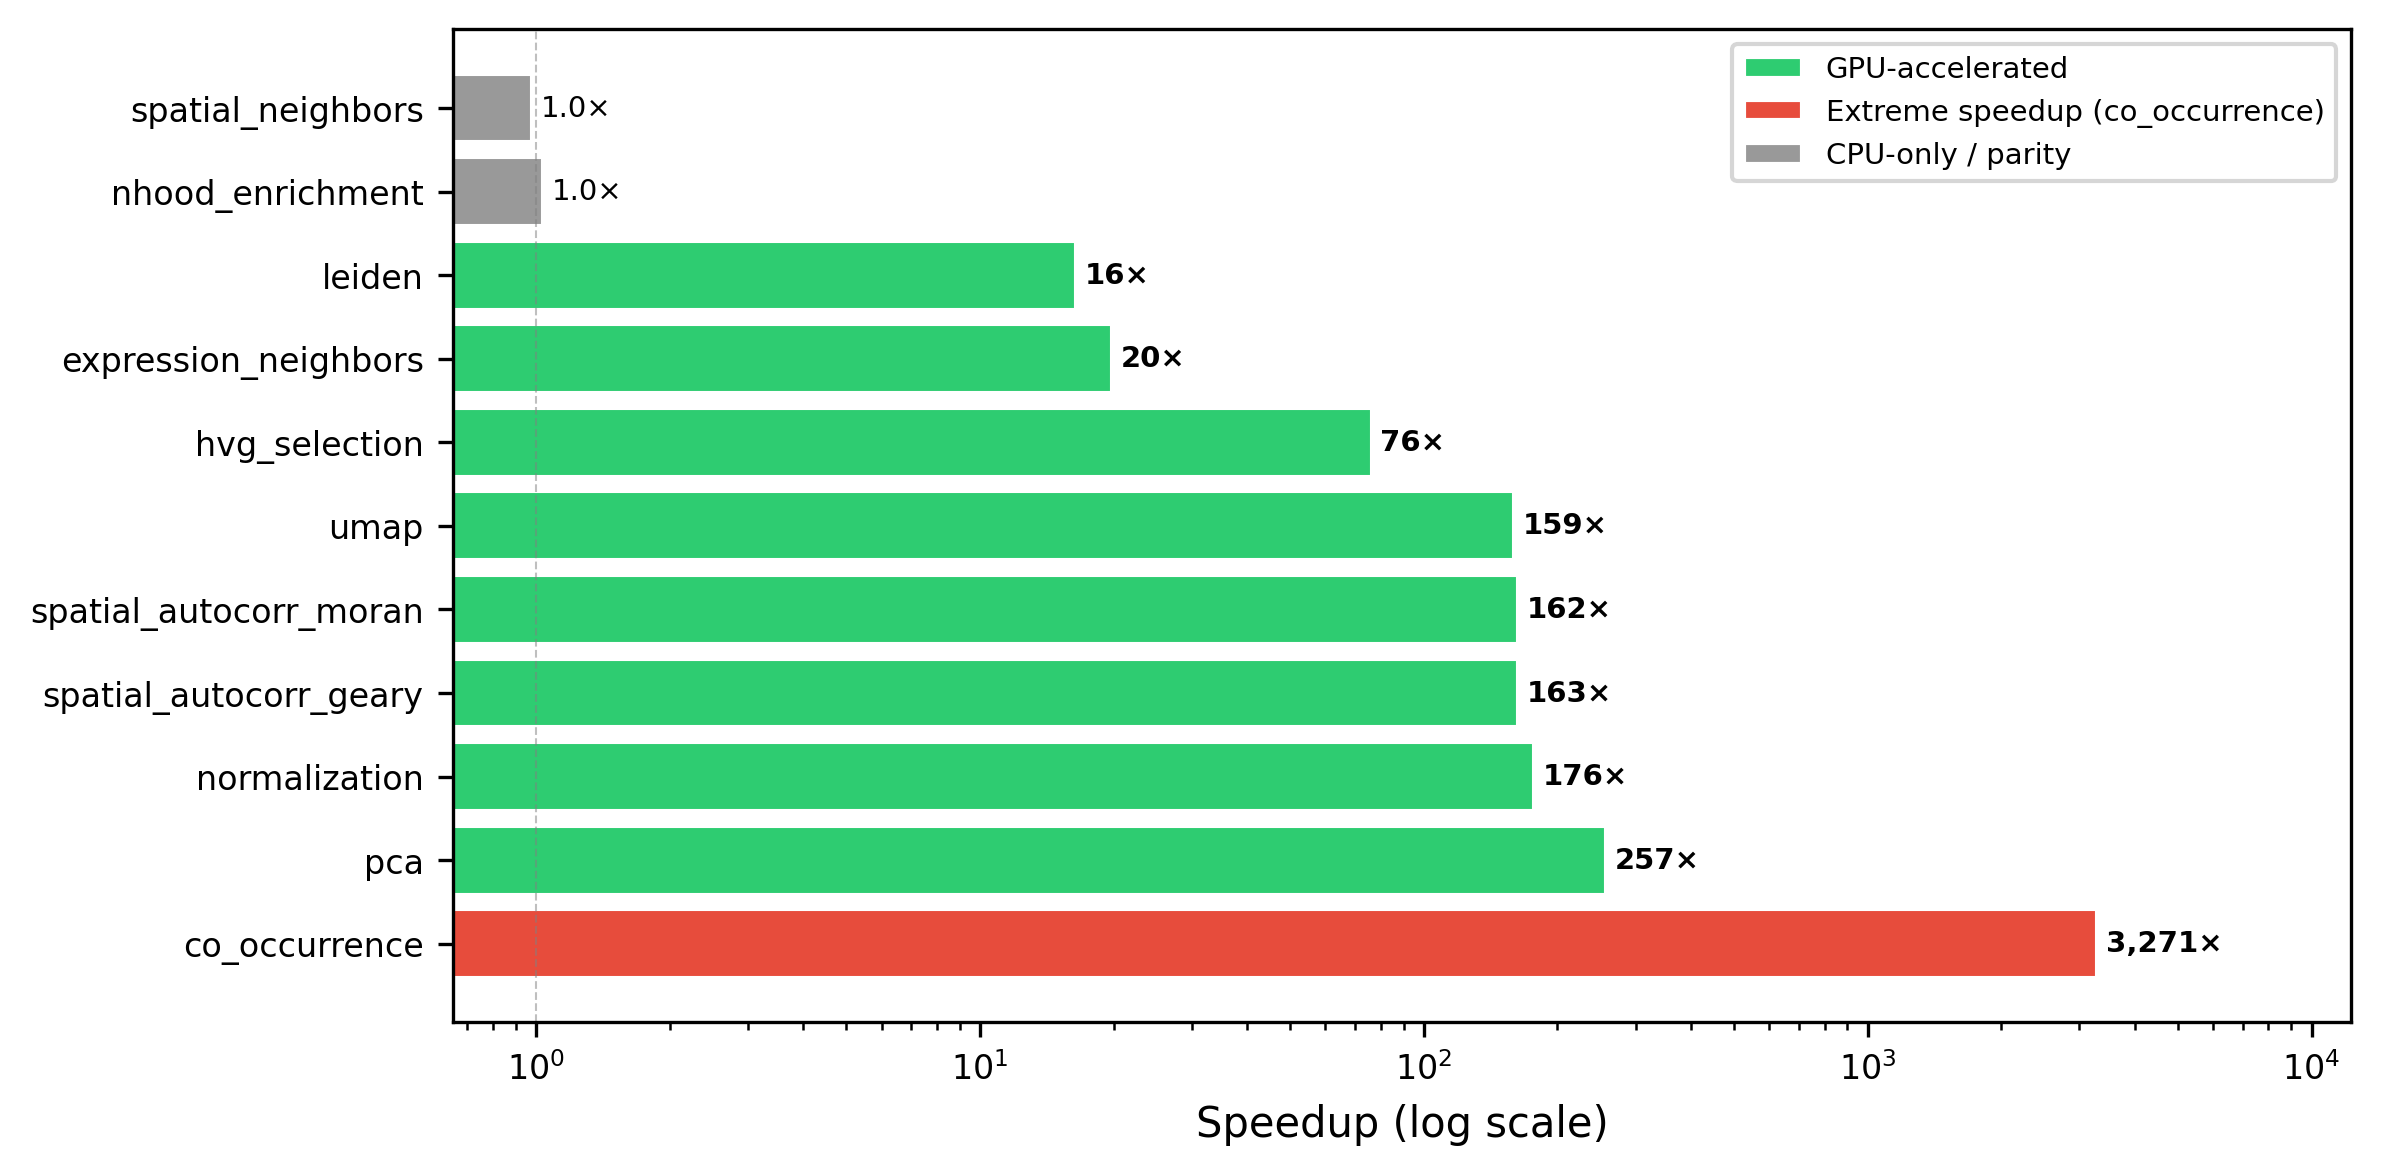
\includegraphics[width=0.85\textwidth,keepaspectratio,alt={Figure 8. Per-step GPU speedup for Visium HD 8 um (393,543 bins). Co-occurrence analysis achieves a 3,272x speedup (CPU: 3,573 s to GPU: 1.09 s), the single largest acceleration measured in this study. Spatial autocorrelation (Moran's I, Geary's C) shows 162-163x speedup. Steps without GPU implementations (spatial\_neighbors, nhood\_enrichment) remain at 1.0x.}]{figures/fig8_spatial_perstep.png}}
\caption{\textbf{Figure 8.} Per-step GPU speedup for Visium HD 8 um
(393,543 bins). Co-occurrence analysis achieves a 3,272x speedup (CPU:
3,573 s to GPU: 1.09 s), the single largest acceleration measured in
this study. Spatial autocorrelation (Moran's I, Geary's C) shows
162-163x speedup. Steps without GPU implementations (spatial\_neighbors,
nhood\_enrichment) remain at 1.0x.}
\end{figure}

Other large GPU advantages on HD 8 um included PCA (257x), normalisation
(176x), spatial autocorrelation (162-163x), and UMAP (159x). Leiden
clustering achieved a 16x speedup, and k-NN graph construction achieved
20x.

\begin{longtable}[]{@{}lrrr@{}}
\caption{\textbf{Table 9.} Per-step wall time and GPU speedup for
spatial-specific operations on Visium HD 8 um (393,543 bins), the
platform showing the largest overall speedup. Steps labelled
``CPU-only'' in the Speedup column lack a GPU implementation in
rapids-singlecell 0.14.1; the ``GPU (s)'' value for those rows reports
the wall time of the CPU fallback executed transparently inside the GPU
pipeline, not a GPU-accelerated
measurement.}\label{tbl:spatial_steps}\tabularnewline
\toprule\noalign{}
Step & CPU (s) & GPU (s) & Speedup \\
\midrule\noalign{}
\endfirsthead
\toprule\noalign{}
Step & CPU (s) & GPU (s) & Speedup \\
\midrule\noalign{}
\endhead
\bottomrule\noalign{}
\endlastfoot
Co-occurrence & 3,573 & 1.09 & 3,272x \\
PCA & 72.8 & 0.28 & 257x \\
Normalisation & 0.65 & 0.004 & 176x \\
Moran's I & 47.9 & 0.30 & 162x \\
Geary's C & 47.4 & 0.29 & 163x \\
UMAP & 194.3 & 1.22 & 159x \\
HVG selection & 0.94 & 0.012 & 76x \\
Expression neighbours & 39.4 & 2.00 & 20x \\
Leiden clustering & 19.2 & 1.17 & 16x \\
Spatial neighbours & 55.9 & 57.4 & 1.0x (CPU-only) \\
Nhood enrichment & 11.8 & 11.4 & 1.0x (CPU-only) \\
\end{longtable}

Visium HD 2 um showed a lower overall speedup (10.8x) despite a similar
bin count (389,492) because co-occurrence analysis was skipped
(\textgreater500 clusters exceeded the O(k\^{}2) memory threshold).
Without this step, UMAP dominated the GPU pipeline time (92x speedup,
but consuming 92\% of the 97 s total GPU time).

On Visium v1, the modest 1.7x overall speedup reflects the small dataset
size (2,695 spots): GPU kernel launch overhead is not amortised, and
CPU-only steps (spatial neighbours, ligand-receptor) dominate.

Three pipeline steps lacked GPU implementations and constituted the GPU
pipeline's primary bottleneck: spatial neighbours (Delaunay
triangulation via scipy.spatial, \textasciitilde55 s on all HD
platforms), neighbourhood enrichment (CPU-only), and ligand-receptor
interaction (CPU-only, Visium v1 only). Spatial neighbours alone
represented 57-73\% of total GPU pipeline time on HD platforms.

\subsubsection{Spatial concordance: near-perfect for spatial statistics,
divergent for clustering at high
resolution}\label{spatial-concordance-near-perfect-for-spatial-statistics-divergent-for-clustering-at-high-resolution}

Spatial autocorrelation concordance was near-perfect across all
platforms (Table 10, Fig. 9).

\pandocbounded{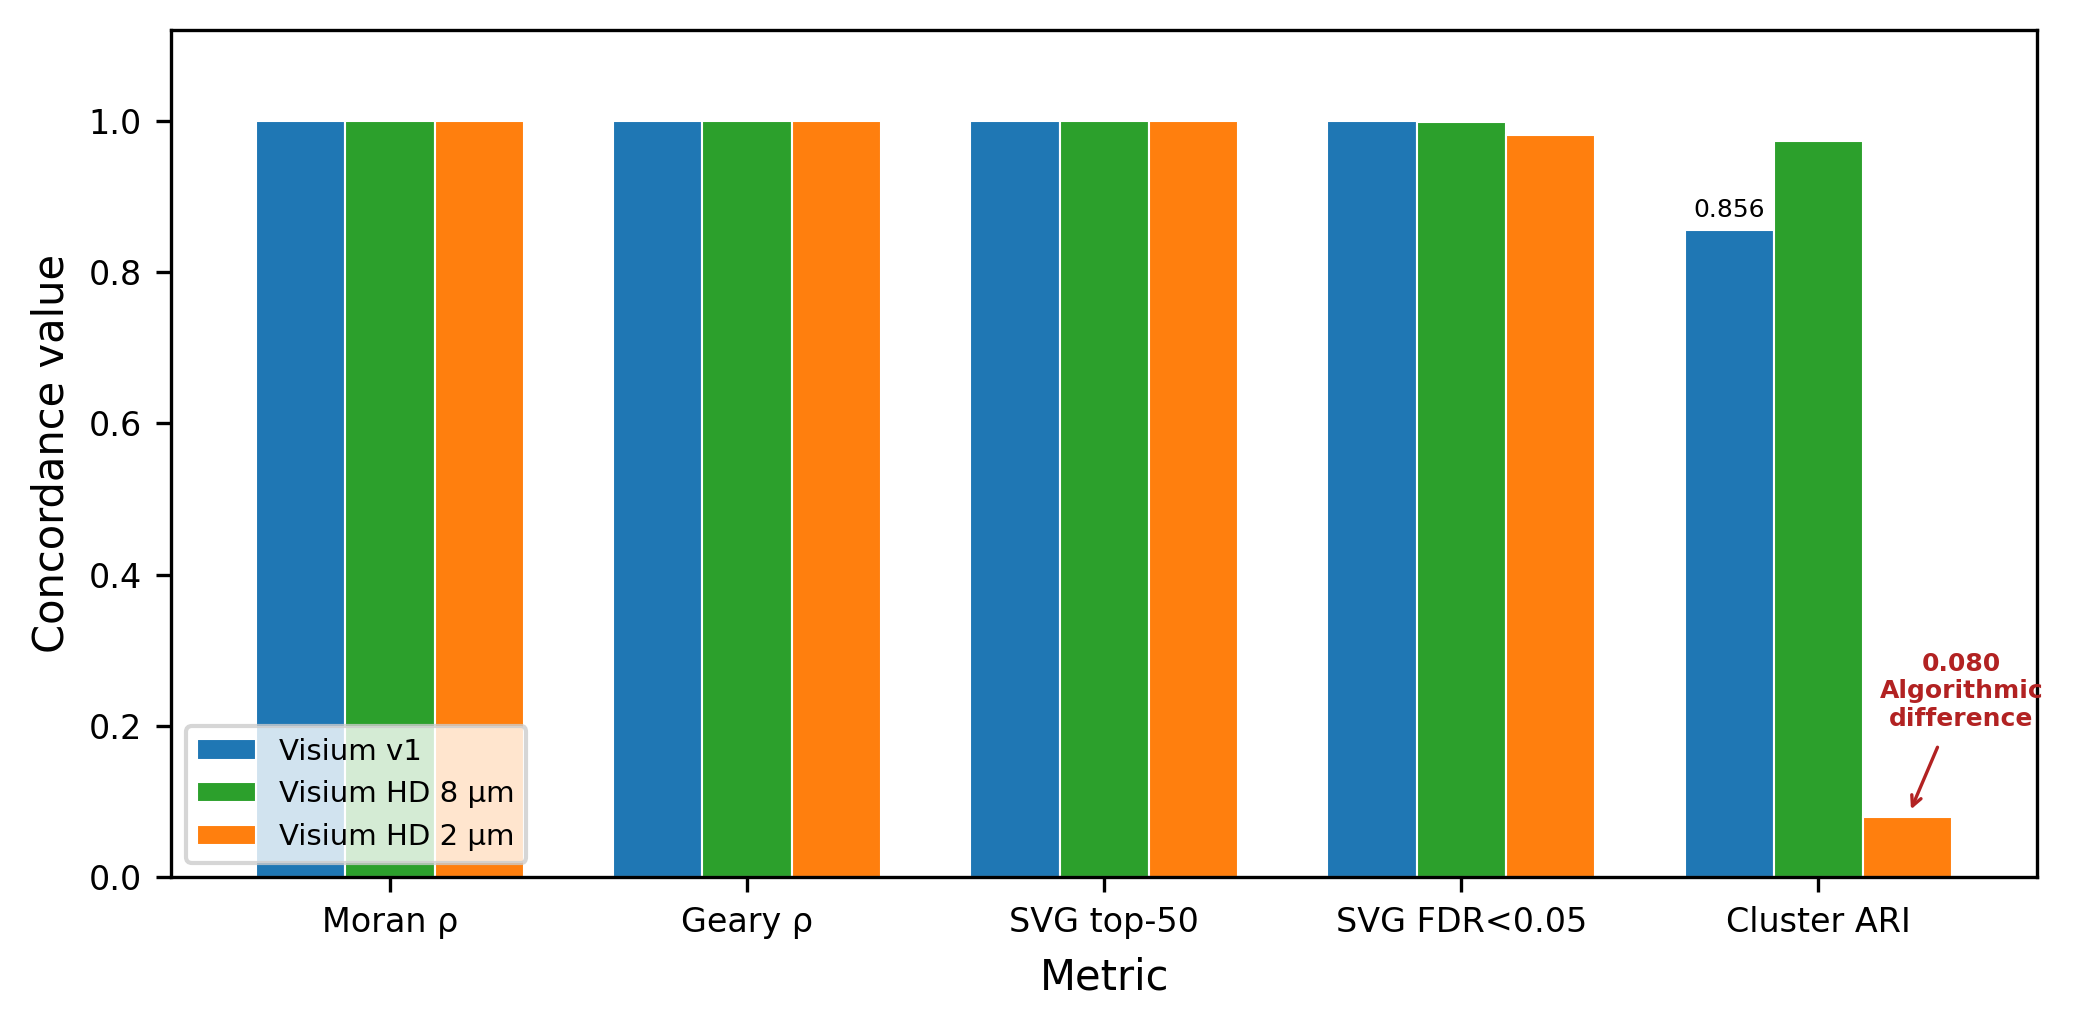
\includegraphics[width=0.85\textwidth,keepaspectratio,alt={Figure 9. Concordance between CPU and GPU spatial analysis pipelines across three Visium platforms. Spatial autocorrelation statistics (Moran's I, Geary's C) show near-perfect agreement (Spearman rho \textgreater= 0.9995). SVG Jaccard overlap of the top 50 genes equals 1.0 for all platforms. Cluster concordance (ARI) degrades at HD 2 um resolution (0.080) due to algorithmic differences between cugraph and leidenalg Leiden implementations at high granularity.}]{figures/fig9_spatial_concordance.png}}
Moran's I and Geary's C Spearman correlations between CPU and GPU
exceeded 0.9995 in all cases. The top-50 spatially variable genes were
identical (Jaccard = 1.0) across all three platforms, confirming that
GPU-accelerated spatial autocorrelation produces scientifically
equivalent results. At the FDR \textless{} 0.05 threshold, SVG overlap
remained high: 100\% (Visium v1), 99.9\% (HD 8 um), and 98.2\% (HD 2
um).

\begin{longtable}[]{@{}lrrr@{}}
\caption{\textbf{Table 10.} Spatial concordance between CPU and GPU
pipelines. SVG Jaccard reports the overlap of top-N spatially variable
genes ranked by Moran's
I.}\label{tbl:spatial_concordance}\tabularnewline
\toprule\noalign{}
Metric & Visium v1 & HD 8 um & HD 2 um \\
\midrule\noalign{}
\endfirsthead
\toprule\noalign{}
Metric & Visium v1 & HD 8 um & HD 2 um \\
\midrule\noalign{}
\endhead
\bottomrule\noalign{}
\endlastfoot
Moran's I Spearman rho & 1.0000 & 0.9999 & 1.0000 \\
Geary's C Spearman rho & 1.0000 & 0.9995 & 0.9999 \\
SVG Jaccard (top 50) & 1.000 & 1.000 & 1.000 \\
SVG Jaccard (FDR \textless{} 0.05) & 1.000 & 0.999 & 0.982 \\
Cluster ARI & 0.856 & 0.974 & 0.080 \\
Cluster NMI & 0.892 & 0.940 & 0.667 \\
N clusters (CPU / GPU) & 16 / 15 & 7 / 3 & 2,559 / 538 \\
\end{longtable}

Expression-based Leiden clustering showed platform-dependent
concordance. On Visium v1 (ARI = 0.856, NMI = 0.892) and HD 8 um (ARI =
0.974, NMI = 0.940), concordance was high, consistent with the scRNA-seq
results. However, on HD 2 um, clustering diverged substantially (ARI =
0.080, NMI = 0.667): the CPU pipeline identified 2,559 clusters while
the GPU pipeline found 538. This 4.75x difference in cluster granularity
arises from algorithmic differences between the leidenalg (CPU) and
cuGraph (GPU) Leiden implementations, which are amplified at high
resolution where the graph has many near-degenerate partitions.
Subsampling from 6.3 million to 389,492 bins also disrupts spatial
contiguity, compounding the effect. This is a known limitation of
comparing stochastic graph-partitioning algorithms across
implementations, not a deficiency of GPU computation per se.

\subsubsection{Memory usage is modest across spatial
platforms}\label{memory-usage-is-modest-across-spatial-platforms}

Peak GPU VRAM was 12.9 GB on Visium v1 and plateaued at 22.6 GB for both
HD platforms (Table 8), well within the RTX 4090's 24 GB capacity. CPU
RAM ranged from 1.3 GB (Visium v1) to 10.8 GB (HD 2 um). These modest
requirements suggest that spatial benchmarks at full Visium HD
resolution (6.3M bins at 2 um) would fit comfortably within DGX H100
memory.

\section{Discussion}\label{discussion}

Our benchmark demonstrates that rapids-singlecell on NVIDIA H100 GPUs
delivers consistent, large-magnitude speedups over Scanpy for the
standard scRNA-seq analysis pipeline, with high biological concordance
and practical scalability to nearly 12 million cells on a single DGX
H100 node. The extension to spatial transcriptomics shows that GPU
advantages are even more pronounced for spatial-specific operations,
with co-occurrence analysis achieving over three orders of magnitude
speedup. These results reveal several important insights about
GPU-accelerated single-cell analysis that merit detailed discussion.

The fundamental constraint underlying our results is that GPU speedup is
inherently operation-specific and highly dependent on the computational
structure of each step. Normalisation and neighbour graph construction
represent ideal GPU workloads, achieving speedups of 88-329x and 44-88x
respectively, because they involve high arithmetic intensity and are
trivially parallelisable across many data elements. In contrast, data
loading from disk and Leiden clustering on small graphs show no GPU
advantage or even a CPU advantage, but for different reasons. For data
loading the culprit is not bandwidth: at sub-gigabyte dataset sizes PCIe
Gen5 (128 GB/s) is far from saturated and the transfer itself completes
in milliseconds; what dominates the GPU-side cost is the fixed overhead
of CUDA context initialisation and RMM pool allocation, and our pipeline
additionally routes \texttt{h5py}-based reads through CPU RAM rather
than via GPU Direct Storage. Leiden clustering on small graphs is
limited by low arithmetic intensity: consistent with the roofline model
\citep{Williams2009}, cuGraph's constant-time overhead exceeds CPU's
short runtime when the graph has few nodes, and the GPU compute units
are not saturated. This heterogeneous speedup landscape has important
practical implications for practitioners: GPU acceleration is most
valuable for large datasets where the compute-heavy operations dominate
overall runtime, whereas on small datasets the overhead of GPU
operations may outweigh their benefits.

This step-level heterogeneity extends into multi-GPU scaling behaviour.
The relatively modest 12\% improvement from 2 to 8 GPUs at 1.3M cells
reflects a fundamental constraint imposed by pipeline structure: only
PCA and neighbour graph construction exploit distributed GPU
computation, while the remaining 95\% of wall time is spent on
inherently sequential CPU preprocessing or single-GPU operations. This
imbalance represents a classic manifestation of Amdahl's law
\citep{Amdahl1967}, where the non-parallelised fraction dominates
overall speedup. Future frameworks could address this bottleneck by
distributing preprocessing operations (e.g., chunked QC and
normalisation across GPUs) and parallelising Leiden clustering across
partitions, but such changes would require substantial modifications to
the existing Scanpy architecture. A practical consequence for resource
allocation follows from this constraint: because the marginal speedup of
adding GPUs to a single run is only approximately 12\%, a DGX H100 node
is more efficiently utilised as eight independent single-GPU workers
running concurrent analyses (yielding near-linear throughput scaling in
the number of concurrent studies) than as an eight-way worker for one
analysis at a time. This is a non-obvious but important takeaway for
groups operating shared GPU infrastructure: the capital-intensive DGX
platform delivers its greatest return when treated as a cluster of eight
H100 workstations, not as one 8xH100 supercomputer.

Related to this, most of the practical value of the GPU speedup is
accessible without a DGX at all. At dataset sizes below 500,000 cells
the full standard pipeline fits on a single H100 GPU, and the
memory-optimised variant described here extends single-GPU feasibility
to 1.3M cells and beyond. Single H100 GPUs are readily rentable on
commercial cloud platforms at approximately USD 2 to 4 per hour, so the
120x speedup at 1.3M cells reported here (reducing a 14.5-hour CPU
analysis to 7.3 minutes) translates to well under one dollar of compute
rental for an entire atlas-scale analysis. Access to a full DGX is
therefore not a prerequisite for adopting these methods; the results are
directly relevant to individual researchers and small groups with
pay-as-you-go cloud budgets.

The biological outputs of GPU and CPU pipelines show high agreement
despite computing on fundamentally different architectures and hardware.
The perfect concordance on HVG selection (Jaccard = 1.000) and PCA
loadings (Spearman rho = 1.000) reflects the deterministic nature of
these operations given identical numerical inputs. The adjusted Rand
indices for Leiden clustering range from 0.908 to 0.963 across different
resolutions, entirely consistent with the algorithm's inherent
stochasticity across implementations (igraph vs cuGraph) and with
published benchmarks of clustering variability in scRNA-seq workflows
\citep{Duo2020}. Floating-point non-associativity in GPU parallel
reductions contributes negligibly to observed differences, as the
dominant source of variation is the Leiden algorithm's non-deterministic
vertex ordering. This level of concordance is reassuring for
practitioners: it indicates that GPU-accelerated and CPU-based analyses
remain interchangeable for biological interpretation and conclusions.

Perhaps most importantly, our findings reveal that CPU-side memory
pressure during preprocessing, not GPU VRAM, is the binding constraint
on scalability at extreme scale. This challenges the common intuition
that GPU memory availability limits GPU-accelerated analysis. At the
maximum testable scale of 11.9 million cells, aggregate GPU VRAM
remained flat at 49 GB (7.6\% of the 640 GB total) while stable peak CPU
RAM reached 535 GB. Critically, the 12M-cell failure did not occur
because CPU RAM was exhausted on average (535 GB is only 30\% of the 1.8
TB job allocation): it occurred because transient memory spikes during
individual preprocessing operations briefly multiplied the working set
past the SLURM cgroup limit (Table 6), notably during Leiden graph
construction and the duplication of \texttt{adata.raw} that Scanpy's DE
backend requires. The bottleneck is therefore not ``RAM being full'' in
the usual sense but a set of short-lived peaks that the scanpy
preprocessing stack is structured to create. Substantial further gains
in capacity could be realised through preprocessing frameworks that
avoid these transient peaks (e.g., reference-only \texttt{adata.raw},
streaming Leiden on partitions, chunked sparse-to-dense transforms),
since GPU VRAM remains heavily underutilised even at near-maximum cell
counts. The capacity limit is more accurately described as a function of
cells x HVGs rather than cell count alone, because the dense scaled
matrix materialised during preprocessing must occupy one contiguous CPU
allocation of n x HVGs x 4 bytes; with 2,000 HVGs this suggests 20M
cells at 1,000 HVGs and 4M cells at 5,000 HVGs as linear-extrapolation
operating points. Our ScaleSC-inspired chunked variant indeed reduced
aggregate VRAM by a factor of five (49 GB to 10 GB) without improving
the cell limit, which further underlines that GPU memory is not the
binding resource in current single-cell workflows.

Pseudo-bulk differential expression represents the optimal balance
between computational efficiency and statistical rigour. Our DE
benchmark confirms that pseudo-bulk aggregation is not merely a
statistical best practice (it avoids pseudoreplication and properly
accounts for inter-donor variability \citep{Squair2021}) but also a
computational optimisation, reducing runtime by 44x relative to
cell-level t-test. GPU acceleration of cell-level DE provides moderate
speedups (3-7x) but is ultimately limited by the I/O cost of converting
sparse matrices to dense gene chunks. Within cell-level tests on GPU the
Wilcoxon rank-sum test actually outperformed the t-test (826 vs 1,656
s), a counterintuitive result that reflects the fact that CuPy's
\texttt{argsort} maps efficiently onto sparse data whereas the t-test
requires dense mean and variance tensors. Beyond these practical
considerations, the use of pseudo-bulk becomes essential when
interpreting results at scale: at 3.4 million cells, p-values from
cell-level tests become uninformative because virtually every gene
reaches statistical significance due to the enormous sample size. Effect
sizes (log-fold-changes) become the primary quantity of interest, and
pseudo-bulk methods coupled with proper count-based models (DESeq2,
edgeR) are the gold standard for multi-donor experiments
\citep{Squair2021}. For contemporary single-cell studies, pseudo-bulk
should therefore be the default approach on both statistical and
computational grounds.

Beyond scRNA-seq, the extension to spatial transcriptomics demonstrates
that GPU acceleration becomes increasingly impactful for computationally
intensive spatial statistics. The 3,272x speedup achieved for
co-occurrence analysis on Visium HD 8 um data is, to our knowledge, the
largest GPU speedup reported for any spatial transcriptomics operation,
reflecting the O(n\^{}2) algorithmic complexity of the CPU
implementation which the GPU effectively parallelises across thousands
of bins and spatial distance intervals simultaneously. Spatial
autocorrelation statistics (Moran's I, Geary's C) achieved similarly
impressive speedups of 162-170x with near-perfect numerical concordance
(rho \textgreater= 0.9995), meaning that scientists can obtain identical
rankings of spatially variable genes in seconds rather than minutes. The
remaining CPU-only operations (spatial neighbours computation via
Delaunay triangulation, neighbourhood enrichment, and ligand-receptor
analysis) represent clear opportunities for future GPU-native
implementations and likely harbour substantial additional speedup
potential.

A notable finding from spatial analysis concerns clustering at extreme
resolution. The dramatic divergence at Visium HD 2 um (ARI = 0.080) is
not specific to GPU versus CPU comparison; rather, it reflects the
fundamental sensitivity of stochastic graph-partitioning algorithms to
implementation details when the solution landscape contains many
near-degenerate partitions. At 389,492 spatial bins with resolution
parameter 0.1, local optima abound, and the leidenalg (CPU) and cuGraph
(GPU) implementations explore this landscape through different vertex
orderings and local heuristics. This observation suggests that users
working at ultra-high spatial resolution should not rely on a single run
of any Leiden implementation, but instead employ consensus clustering
approaches or spatial-aware alternative methods that explicitly account
for tissue geometry.

Our study contains several limitations that should be considered when
generalising these findings. The scRNA-seq benchmark used a single
biological dataset (mouse brain E18); performance profiles may differ
substantially for datasets with different sparsity patterns, gene
counts, or biological characteristics. Concordance analysis was
performed at 10,000 cells; larger datasets may exhibit different
adjusted Rand index distributions or reveal additional numerical
differences. The stress test employing the memory-optimised pipeline is
mathematically equivalent to but not implementation-identical to the
standard rapids-singlecell workflow, introducing potential differences
in how the optimization generalises to other analyses. Spatial
benchmarks were conducted on a local RTX 4090 workstation rather than
the DGX H100 cluster, precluding measurements of multi-GPU spatial
scaling and benchmarking of the full Visium HD 2 um resolution (6.3
million bins). Scaling analysis was confined to a single DGX H100 node
(1-8 GPUs); we did not benchmark multi-node configurations (e.g., 16
GPUs across two nodes interconnected by InfiniBand) because the
near-flat wall time observed from 2 to 8 GPUs already indicates that the
dominant bottleneck lies in CPU-side preprocessing and single-GPU graph
operations (Leiden, UMAP), neither of which would benefit from
additional nodes and both of which would be further penalised by
inter-node communication latency. Finally, we did not benchmark
integration methods (Harmony, scVI) or multi-sample spatial experimental
designs, which represent important directions for ongoing work.

\section{Conclusions}\label{conclusions}

GPU-accelerated single-cell analysis via rapids-singlecell on NVIDIA
H100 GPUs reduces a 14.5-hour CPU pipeline to 7.3 minutes at 1.3M cells,
with biologically concordant results. The principal scalability
bottleneck is CPU-side preprocessing, not GPU VRAM: a single DGX H100
node processed 11.9M cells while using only 7.6\% of total GPU memory.
Multi-GPU scaling provides modest benefit (12\% at 1.3M cells, 2 to 8
GPUs) due to the dominance of non-GPU-parallelised pipeline phases. For
differential expression, pseudo-bulk aggregation is simultaneously the
fastest (44x vs t-test) and most statistically rigorous approach. For
spatial transcriptomics, GPU acceleration delivers 51.6x end-to-end
speedup on Visium HD, with co-occurrence analysis achieving a 3,272x
speedup and spatial autocorrelation concordance exceeding 0.9995. These
results provide practical guidance for the computational bioinformatics
community as single-cell and spatial datasets grow toward the
billion-cell and billion-bin scales \citep{Regev2017}.

\section{Conflict of Interest}\label{conflict-of-interest}

The authors declare no conflict of interest.

\section{Acknowledgements}\label{acknowledgements}

The computational resources for the scRNA-seq benchmarks were provided
by the UPSCALE/CONVECS DGX H100 cluster at the University of Padova.

\section{Funding}\label{funding}

This study was co-funded by the BIRD 2024/START (SID) programs,
Department of Cardio-Thoracic-Vascular Sciences (DCTV), University of
Padua (PI: Daniele Sabbatini; 2024DCTV1SIDPROGETTI-00183) and by the
Italian Complementary National Plan PNC-I.1 ``Research initiatives for
innovative technologies and pathways in the health and welfare sector''
D.D. 931 of 06/06/2022, ``DARE-DigitAl lifelong pRevEntion'' initiative,
code PNC0000002, CUP: B53C22006450001.

\section{Availability of Data and Software
Code}\label{availability-of-data-and-software-code}

All code, Dockerfiles, SLURM submission scripts, and benchmark result
JSON files are available at
\url{https://github.com/lucavd/2026.scRNA_DGX}.


\bibliographystyle{splncs04}
\bibliography{cibb2026_references}

\end{document}
